\date{}
\title{}
\date{}
\begin{document}
\begin{frame}
    \titlepage
\end{frame}


\makeatletter
\newenvironment<>{btHighlight}[1][]
{\begin{onlyenv}#2\begingroup\tikzset{bt@Highlight@par/.style={#1}}\begin{lrbox}{\@tempboxa}}
{\end{lrbox}\bt@HL@box[bt@Highlight@par]{\@tempboxa}\endgroup\end{onlyenv}}

\newcommand<>\btHL[1][]{%
  \only#2{\begin{btHighlight}[#1]\bgroup\aftergroup\bt@HL@endenv}%
}
\def\bt@HL@endenv{%
  \end{btHighlight}%   
  \egroup %
}
\tikzset{
    btHLbox/.style={
        fill=red!30,outer sep=0pt,inner xsep=1pt, inner ysep=0pt, rounded corners=3pt
    },
}
\newcommand{\bt@HL@box}[2][]{%
  \tikz[#1]{%
    \pgfpathrectangle{\pgfpoint{1pt}{0pt}}{\pgfpoint{\wd #2}{\ht #2}}%
    \pgfusepath{use as bounding box}%
    \node[text width={},draw=none,anchor=base west, btHLbox, minimum height=\ht\strutbox+1pt,#1]{\raisebox{1pt}{\strut}\strut\usebox{#2}};
  }%
}

\lst@CCPutMacro
    \lst@ProcessOther {"2A}{%
      \lst@ttfamily 
         {\raisebox{2pt}{*}}% used with ttfamily
         {\raisebox{2pt}{*}}}% used with other fonts
    \@empty\z@\@empty

\lstdefinelanguage
   [x8664gas]{Assembler}     % add a "x64" dialect of Assembler
   [x86masm]{Assembler} % based on the "x86masm" dialect
   % with these extra keywords:
   {morekeywords={CDQE,CQO,CMPSQ,CMPXCHG16B,JRCXZ,LODSQ,MOVSXD,%
                  POPFQ,PUSHFQ,SCASQ,STOSQ,IRETQ,RDTSCP,SWAPGS,.TEXT,.STRING,.ASCIZ,%
                  BEQ,LW,SW,LB,SB,ADDIU,J,BEQZ,BNEZ,BNE,%
                  MOVUPD,MULPD,MOVSD,MULSD,%
                  SHLADD,MOV,CMP.LT,TBIT.NZ,BR.RET.SPTK.MANY,%
                  ADDQ,POPQ,PUSHQ,RRMOVQ,MRMOVQ,RMMOVQ,IRMOVQ,%
                  <-,LL,SC,ADDI,ADDL,VMOVDQA,ADDQ,CMPL,JB,JBE,MOVL,CLTQ,%
                  MOVW,PUSHW,MOV,ADD,SUB,INT,PUSH,MOV,ADD,REP,MOVSB,%
                  TESTQ,CMPQ,MOVL,MOVQ,ADDQ,JMPQ,XORQ,%
                  LEAQ,LEAL,LEA,RETQ,RET,POPL,POPW,PUSHL,PUSHW,%
                  LEAW,%
                  SUBQ,SYSCALL,.ASCII,CALLQ,MOVSLQ,JMP,ANDQ,SHRQ,MOVB,INCQ,TESTL,XORL,%
                  SHRL,LEAL,SARL,SUBL,IMULL,IMULQ,MOVDQU,PADDD,XORL,%
                  MOVZBL,MOVZB,SHRB,SRAL,SHRL,ANDL,%
                  CMOVNS,SRAL,SRAQ,MOVZBW,MOVZBQ,%
                  PADDW,PADDQ,MODUPS,MOVAPD,%
                  MOVL,RET,.GLOBL,%
		  PAUSE,LFENCE,JMP,%
                  },
    deletekeywords={eax,ebx,sp,si,cx,di,ds,cs,es,fs,dx,ax,bx,al,esi,ebp,ecx,rip,eip,edx,edi,rdi,esp},
    deletekeywords=[2]{size},
    alsoletter={\%},
    alsoother={()},
    emphstyle={\color{violet!50!black}},
    emph={\%rax,\%rbx,\%rcx,\%rdx,\%r8,\%r9,\%r10,\%r11,\%r12,\%r13,\%r14,\%r15,\%eax,\%ebx,\%sp,\%si,\%cx,\%di,\%ds,\%cs,\%es,\%fs,\%dx,\%ax,\%bx,\%al,\%esi,\%ebp,\%ecx,\%rip,\%eip,\%edx,\%edi,\%rdi,\%esp,\%rsp},
    %moreemph={eax,ebx,sp,si,cx,di,ds,cs,es,fs,dx,ax,bx,al,esi,ebp,ecx,rip,eip,edx,edi,rdi,esp},
    morecomment=[l]{\#},
    morecomment=[l]{\/\/},
    morecomment=[s]{/*}{*/},
    sensitive=false,
    keepspaces=true} % et

\lstalias[]{myasm}[x8664gas]{Assembler}

\lstdefinelanguage{JavaScript}{
  keywords={typeof, new, true, false, catch, function, return, null, catch, switch, var, if, in, while, do, else, case, break},
  ndkeywords={class, export, boolean, throw, implements, import, this},
  sensitive=false,
  comment=[l]{//},
  morecomment=[s]{/*}{*/},
  morestring=[b]',
  morestring=[b]"
}

\newcommand{\keywordstyle}{\sourcecodeprolight\bfseries\color{blue!30!black}}
\newcommand{\stringstyle}{\color{blue!20!black}\ttfamily}

\lstset{
    language=C,
    basicstyle=\sourcecodepro\EmptyMapping,
    escapechar=`,
    keywordstyle=\keywordstyle\EmptyMapping,
    identifierstyle=\sourcecodepro\EmptyMapping,
    numberstyle=\small\color{black!70},
    commentstyle=\color{red!60!black}\ttfamily\itshape,
    stringstyle=\color{blue!20!black}\ttfamily,
    ndkeywordstyle=\bfseries\color{blue!30!black},
    upquote=true,
}



\lstdefinestyle{medium}{
    basicstyle=\sourcecodepro\EmptyMapping\fontsize{12}{13}\selectfont,
    keywordstyle=\sourcecodepro\EmptyMapping\fontsize{12}{13}\selectfont\keywordstyle,
}

\lstdefinestyle{small}{
    basicstyle=\sourcecodepro\EmptyMapping\small,
    keywordstyle=\sourcecodepro\EmptyMapping\small\keywordstyle,
}

\lstdefinestyle{smaller}{
    basicstyle=\sourcecodepro\EmptyMapping\fontsize{11}{12}\selectfont,
    keywordstyle=\sourcecodepro\EmptyMapping\fontsize{11}{12}\selectfont\keywordstyle,
}

\lstdefinestyle{size105}{
    basicstyle=\sourcecodepro\EmptyMapping\fontsize{10.5}{11.5}\selectfont,
    keywordstyle=\sourcecodepro\EmptyMapping\fontsize{10.5}{11.5}\selectfont\keywordstyle,
}

\lstdefinestyle{size10}{
    basicstyle=\sourcecodepro\EmptyMapping\fontsize{10}{11}\selectfont,
    keywordstyle=\sourcecodepro\EmptyMapping\fontsize{10}{11}\selectfont\keywordstyle,
}

\lstdefinestyle{size9}{
    basicstyle=\sourcecodepro\EmptyMapping\fontsize{9}{10}\selectfont,
    keywordstyle=\sourcecodepro\EmptyMapping\fontsize{9}{10}\selectfont\keywordstyle,
}
\lstdefinestyle{size8}{
    basicstyle=\sourcecodepro\EmptyMapping\fontsize{8}{9}\selectfont,
    keywordstyle=\sourcecodepro\EmptyMapping\fontsize{8}{9}\selectfont\keywordstyle,
}



\lstdefinestyle{script}{
    basicstyle=\sourcecodepro\EmptyMapping\scriptsize,
    keywordstyle=\sourcecodepro\EmptyMapping\scriptsize\bfseries,
}




\begin{frame}{last time}
    \begin{itemize}
    \item LOAD directives in ELF files
    \item position-independent versus not
    \vspace{.5cm}
    \item x86-64: opcode | mod / reg (or ext. opcode) / r/m | SIB | constants
    \item tables for ModRM and SIB bytes
    \item REX prefix to add extra register bits/mark 64-bit instructions
    \end{itemize}
\end{frame}

\subsection{adding 64-bit}
\usetikzlibrary{arrows.meta,shapes.multipart}

\begin{frame}{what about 64-bit?}
\begin{itemize}
\item adds 8 more registers --- more bits for reg \#?
\item didn't change encoding for existing instructions, so\ldots
\item \myemph{instruction prefix} ``REX''
    \begin{itemize}
    \item 32-bit x86 already had many prefixes
    \end{itemize}
\item also selects 64-bit version of instruction
\end{itemize}
\end{frame}

\begin{frame}{REX prefix}
\begin{tikzpicture}
    \node[draw,rectangle split,rectangle split horizontal, rectangle split parts=5,
        label={north:REX prefix byte}] (rexbyte) {
        {\tt 0100}
        \nodepart{two}
        w
        \nodepart{three}
        r
        \nodepart{four}
        s
        \nodepart{five}
        b
    };
    \node[anchor=north west,align=left] (wExplain) at ([yshift=-5cm,xshift=.5cm]rexbyte.five south) {
        {\tt 1} if 64-bit values ({\tt \%rax}, etc. or from memory)\\
        {\tt 0} if 32-bit values ({\tt \%eax}, etc. or from memory)
    };
    \draw[thick,-Latex] (rexbyte.two south) |- (wExplain.west);
    \node[anchor=south west] (rExplain) at ([yshift=1mm]wExplain.north west) {
        extra bit for ModRM reg field
    };
    \draw[thick,-Latex] (rexbyte.three south) |- (rExplain.west);
    \node[anchor=south west] (sExplain) at ([yshift=1mm]rExplain.north west) {
        extra bit for SIB byte index reg field
    };
    \draw[thick,-Latex] (rexbyte.four south) |- (sExplain.west);
    \node[anchor=south west, align=left] (bExplain) at ([yshift=1mm]sExplain.north west) {
        extra bit for ModRM r/m \\ or SIB base reg field
    };
    \draw[thick,-Latex] (rexbyte.five south) |- (bExplain.west);
\end{tikzpicture}
%\vspace{.5cm}
%\item 4-bit constant 0100
%\item 1-bit ``w'': 1 if 64-bit operands
%\item 1-bit ``r'': extra bit for ModRM register number
%\item 1-bit ``s'': extra bit for SIB index register number
%\item 1-bit ``b'': extra bit for ``r/m'' or SIB index register number 
%    \begin{itemize}
%    \item or modify in-opcode register number
%    \end{itemize}
%\end{itemize}
\end{frame}



\subsection{exercise}
\begin{frame}{64-bit REX exercise (1)}
    \begin{itemize}
    \item \texttt{add \%eax, \%ecx} (Intel: {\tt ADD ecx, eax})
        \begin{itemize}
        \item {\tt 01} (opcode) {\tt c1} (MOD: 11 / REG: 000 (eax) / R\/M: 001 (ecx))
        \end{itemize}
    \item exercise 2a: \texttt{add \%eax, \%r10d} (Intel: {\tt ADD r9d, eax}) = ???
        \begin{itemize}
        \item REX prefix + {\tt 01} + MOD-REG-R/M byte
        \end{itemize}
    \vspace{.5cm}
    \item REX prefix:
        \begin{itemize}
        \item {\tt 0100}
        \item w (is 64-bit values?)
        \item r (extra bit for Reg field)
        \item s (extra bit for SIB index reg)
        \item b (extra bit for R/M or SIB base field)
        \end{itemize}
    \end{itemize}
\end{frame}

\begin{frame}{64-bit REX exercise (2)}
    \begin{itemize}
    \item \texttt{add \%eax, \%ecx} (Intel: {\tt ADD ecx, eax})
        \begin{itemize}
        \item {\tt 01} (opcode) {\tt c1} (MOD: 11 / REG: 000 (eax) / R\/M: 001 (ecx))
        \end{itemize}
    \item exercise 2b: \texttt{add \%rax, \%rcx} (Intel: {\tt ADD rcx, rax}) = ???
        \begin{itemize}
        \item REX prefix + {\tt 01} + MOD-REG-R/M byte
        \end{itemize}
    \vspace{.5cm}
    \item REX prefix:
        \begin{itemize}
        \item {\tt 0100}
        \item w (is 64-bit values?)
        \item r (extra bit for Reg field)
        \item s (extra bit for SIB index reg)
        \item b (extra bit for R/M or SIB base field)
        \end{itemize}
    \end{itemize}
\end{frame}


\subsection{encoding overall}
\begin{frame}{overall encoding}
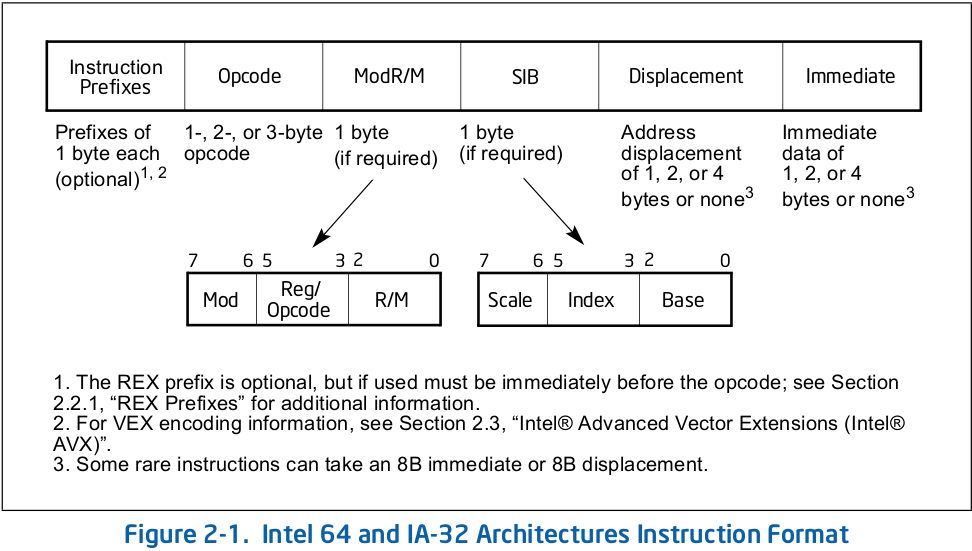
\includegraphics[width=\textwidth]{../x8664-encoding/IntelFig21}
\end{frame}


\subsection{misc prefixes}

\begin{frame}<1>[label=prefixes]{instruction prefixes}
    \begin{itemize}
    \item REX (64-bit and/or extra register bits)
    \item VEX (SSE/AVX instructions; other new instrs.)
    \item operand/address-size change (64/32 to 16 or vice-versa)
    \item {\tt LOCK} --- synchronization between processors
    \item \myemph<2>{{\tt REPNE/REPNZ/REP/REPE/REPZ} --- turns instruction into loop}
    \item segment overrides
    \end{itemize}
\end{frame}




\subsection{examples}

\begin{frame}[fragile,label=x86ex1]{x86 encoding example (1)}
    \begin{itemize}
    \item \lstinline|pushq %rax| encoded as {\tt 50}
        \begin{itemize}
        \item 5-bit opcode {\tt 01010} plus 3-bit register number {\tt 000} \\
        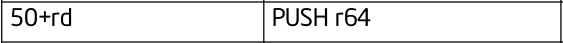
\includegraphics[width=0.4\textwidth]{../x8664-encoding/intel-manual-push-ex1}
        \end{itemize}
    \item \lstinline|pushq %r13| encoded as {\tt 41 55}
        \begin{itemize}
        \item {\tt 41}: REX prefix {\tt 0010} (constant), w:{\tt 0}, r:{\tt 0}, s:{\tt 0}, b:{\tt \color{blue!80!black}{1}}
        \item w = {\tt 0} because push is never 32-bit in 64-bit mode
        \item {\tt 55}: 5-bit opcode {\tt 01010}; 3-bit reg \# {\tt \color{green!80!black}{101}}
        \item 4-bit reg \# {\tt \color{blue!80!black}{1}\color{green!80!black}{101}} = 13
        \end{itemize}
    \end{itemize}
\end{frame}

\begin{frame}[fragile,label=x86ex2]{x86 encoding example (2)}
    \begin{itemize}
    \item \lstinline|addl 0x12345678(%rax,%rbx,2), %ecx|
    \item {\tt 03}: opcode --- add r/m32 into r32 
        \begin{itemize}
        \item
            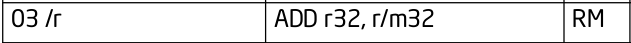
\includegraphics[width=0.4\textwidth]{../x8664-encoding/intel-manual-addl-ex1.png}
            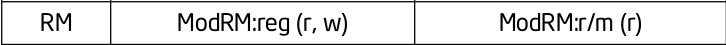
\includegraphics[width=0.4\textwidth]{../x8664-encoding/intel-manual-addl-ex2.png}
        \end{itemize}
    \item {\tt 8c}: ModRM: mod = {\tt 10}; reg = {\tt 001}, r/m: {\tt 100}
        \begin{itemize}
        \item reg = {\tt 001} = {\tt \%ecx} (table)
        \item SIB byte + 32-bit displacement (table)
        \end{itemize}
    \item {\tt 58}: SIB: scale = {\tt 01}, index = {\tt 011}, base = {\tt 000}
        \begin{itemize}
        \item index {\tt 011} = {\tt \%rbx}; base {\tt 000} = {\tt \%rax};
        \end{itemize}
    \item {\tt 78 56 32 12}: 32-bit constant {\tt 0x12345678}
    \end{itemize}
\end{frame}

\begin{frame}[fragile,label=x86ex3]{x86 encoding example (3)}
    \begin{itemize}
    \item \lstinline|addq 0x12345678(%r10,%r11,2), %rax|
    \item {\tt 4b}: REX prefix {\tt 0100}+w:{\tt \myemph<2>{1}}, r:{\tt \textcolor{violet!80!black}{\myemph<3>{0}}}, s:{\tt \textcolor{blue!80!black}{\myemph<4>{1}}}, b:{\tt \textcolor{green!80!black}{\myemph<5>{1}}}
    \item {\tt 03}: opcode --- add r/m64 to r64 (with \myemph<2>{REX.w})
    \item {\tt 84}: ModRM: mod = {\tt 10}; reg = {\tt 000}, r/m: {\tt 100}
        \begin{itemize}
        \item reg = {\tt \textcolor{violet!80!black}{\myemph<3>{0}}000} = \%rax
        \item SIB byte + 32-bit displacement (table)
        \end{itemize}
    \item {\tt 5a}: SIB: scale = {\tt 01}, index = {\tt 011}, base = {\tt 010}
        \begin{itemize}
        \item with REX: index = {\tt \textcolor{blue!80!black}{\myemph<4>{1}}011} (11), base = {\tt \textcolor{green!80!black}{\myemph<5>{1}}010} (10)
        \end{itemize}
    \item {\tt 78 56 32 12}: 32-bit constant {\tt 0x12345678}
    \end{itemize}
\end{frame}

\begin{frame}[fragile,label=x86ex4]{x86 encoding example (4)}
    \begin{itemize}
    \item \lstinline|movq %fs:0x10,%r13|
    \item {\tt 64}: FS segment override
    \item {\tt 48}: REX: {\tt w}: 1 (64-bit), {\tt r}: \textcolor{violet!80!black}{\tt \myemph<2>{1}}, {\tt s}: \textcolor{blue!80!black}{\tt \myemph<3>{0}}, {\tt b}: \textcolor{green!80!black}{\tt \myemph<4>{0}}
    \item {\tt 8b}: opcode for MOV memory to register
    \item {\tt 2c}: ModRM: mod = {\tt 00}, reg = {\tt 101}, r/m: {\tt 100}
        \begin{itemize}
        \item with REX: reg = {\tt \textbf{\textcolor{violet!80!black}{\myemph<2>{1}}}101} [\%r12]; r/m = {100} (SIB follows)
        \end{itemize}
    \item {\tt 25}: SIB: scale = {\tt 00}; index = {\tt (\textcolor{blue!80!black}{\myemph<3>{0}})100}; base = {\tt (\textcolor{green!80!black}{\myemph<4>{0}})101}
        \begin{itemize}
        \item no register/no register in table
        \end{itemize}
    \item {\tt 10 00 00 00}: 4-byte constant {\tt 0x10}
    \end{itemize}
\end{frame}




\subsection{some impossible instructions}

\begin{frame}[fragile,label=x8664impos]{x86-64 impossibilities}
\lstset{
    language=myasm,
    style=small,
    moredelim={**[is][\sout<all:1>]{~sout~}{~endsout~}},
}
    \begin{itemize}
    \item \myemph{illegal}: \lstinline|~sout~movq 0x12345678ab(%rax), %rax~endsout~|
        \begin{itemize}
        \item maximum 32-bit displacement
        \item \lstinline|movq 0x12345678ab, %rax| okay
            \begin{itemize}
            \item extra {\tt mov} opcode for {\tt \%rax} only
            \end{itemize}
        \end{itemize}
    \item \myemph{illegal}: \lstinline|~sout~movq $0x12345678ab, %rbx~endsout~|
        \begin{itemize}
        \item maximum 32-bit constant
        \item \lstinline|movq $0x12345678ab, %rax| okay
        \end{itemize}
    \item \myemph{illegal}: \lstinline|~sout~pushl %eax~endsout~|
        \begin{itemize}
        \item no 32-bit push/pop in 64-bit mode
        \item but 16-bit allowed (operand size prefix byte {\tt 66})
        \end{itemize}
    \item \myemph{illegal}: \lstinline|~sout~movq (%rax, %rsp), %rax~endsout~|
        \begin{itemize}
        \item cannot use \lstinline|%rsp| as index register
        \item \lstinline|movq (%rsp, %rax), %rax| okay
        \end{itemize}
    \end{itemize}
\end{frame}



\subsection{position-independence} 
\begin{frame}[fragile,label=picVNot]{position dependence}
\begin{itemize}
\item two ways of encoding addresses in x86-64 assembly:
    \begin{itemize}
    \item address in little endian (typically 32-bits --- limit on executable size)
    \item difference between address and \%rip (next instruction address)
    \end{itemize}
\end{itemize}
\hrule
{\tt
\begin{tabular}{l|l}
movb label, \%al & 8a 04 25 {\normalfont\it label's addr (32 bit)} \\
jmp *label & ff 24 25 {\normalfont\it label's addr (32 bit)} \\
movb label(\%rip), \%al & 8a 05 {\normalfont\it \%rip - label's addr (32 bit)} \\
jmp label & e9 {\normalfont\it \%rip - label's addr (32 bit)} \\
\end{tabular}
}
how to know which? --- check manual
\end{frame}


\subsection{PIC: which should be exercise?}
\begin{frame}{position-independence: which to use?}
\begin{itemize}
\item suppose we're inserting ``evil'' code \\
at changing addresses in executable's memory
\item which of the following do we want absolute encoding for? \\
(i.e. which would absolute encoding be easier than relative)
    \begin{itemize}
    \item A. address of a jump from evil code to function at fixed loc in executable
    \item B. address of a jump in a loop in the ``evil'' code
    \item C. address of a string in the ``evil'' code
    \item D. address of a string in the executable
    \end{itemize}
\end{itemize}
\end{frame}


\begin{frame}{RE2 homework}
\end{frame}

\section{running example}
\begin{frame}[fragile]{running example}
\begin{Verbatim}[fontsize=\small]
$ file mystery
mystery: ELF 64-bit LSB pie executable, x86-64,
version 1 (SYSV), dynamically linked,
interpreter /lib64/ld-linux-x86-64.so.2,
BuildID[sha1]=9819a3cfb39d01ad2a376c54318f104139422a8f,
for GNU/Linux 3.2.0, stripped
\end{Verbatim}
\begin{itemize}
\item LSB = little endian
\item pie = position-independent executable
\item interpreter = program that loads this
\end{itemize}
\end{frame}

\begin{frame}[fragile]{aside: file(1)}
\begin{Verbatim}[fontsize=\small]
$ man file
FILE(1)                      General Commands Manual                    FILE(1)

NAME
       file — determine file type

....
\end{Verbatim}
\hrule
\begin{itemize}
\item looks for ``magic numbers'' near beginning of file data
\item hand-managed database of common patterns
\end{itemize}
\end{frame}

\begin{frame}[fragile]{from file's source}
\begin{Verbatim}[fontsize=\scriptsize]
0   name        elf-le
>16 leshort     0       no file type,
!:mime  application/octet-stream
>16 leshort     1       relocatable,
!:mime  application/x-object
>16 leshort     2       executable,
!:mime  application/x-executable
>16 leshort     3       ${x?pie executable:shared object},

...
0   string      \177ELF     ELF
!:strength *2
>4  byte        0       invalid class
>4  byte        1       32-bit
>4  byte        2       64-bit
>5  byte        0       invalid byte order
>5  byte        1       LSB
>>0 use     elf-le
>5  byte        2       MSB
>>0 use     \^elf-le
>7  byte        0       (SYSV)
\end{Verbatim}
\end{frame}


\section{finding strings}

\begin{frame}[fragile]{finding strings}
\begin{Verbatim}[commandchars=~\{\},fontsize=\fontsize{9}{10}]
$ hexdump -c mystery
00000000  7f 45 4c 46 02 01 01 00  00 00 00 00 00 00 00 00  |.ELF............|
00000010  03 00 3e 00 01 00 00 00  c0 60 00 00 00 00 00 00  |..>......`......|
00000020  40 00 00 00 00 00 00 00  08 5e 03 00 00 00 00 00  |@........^......|
00000030  00 00 00 00 40 00 38 00  0d 00 40 00 1e 00 1d 00  |....@.8...@.....|
~textit{[... many more lines ...]}
00000e60  00 5f 49 54 4d 5f 64 65  72 65 67 69 73 74 65 72  |._ITM_deregister|
00000e70  54 4d 43 6c 6f 6e 65 54  61 62 6c 65 00 5f 5f 67  |TMCloneTable.__g|
00000e80  6d 6f 6e 5f 73 74 61 72  74 5f 5f 00 5f 49 54 4d  |mon_start__._ITM|
00000e90  5f 72 65 67 69 73 74 65  72 54 4d 43 6c 6f 6e 65  |_registerTMClone|
00000ea0  54 61 62 6c 65 00 77 61  64 64 63 68 00 63 6c 65  |Table.waddch.cle|
00000eb0  61 72 6f 6b 00 6e 6f 65  63 68 6f 00 6d 76 70 72  |arok.noecho.mvpr|
~textit{[... many more lines ...]}
\end{Verbatim}
\end{frame}

\begin{frame}{exercise: heuristic?}
    \begin{itemize}
    \item could scan through pages of hexdump for something interesting\ldots
    \vspace{.5cm}
    \item good heuristic for automating this process?
    \end{itemize}
\end{frame}

\begin{frame}[fragile]{strings utility (1)}
\begin{Verbatim}[fontsize=\fontsize{9}{10}]
$ strings mystery
/lib64/ld-linux-x86-64.so.2
*7lT1
A9B*
m8m7
_ITM_deregisterTMCloneTable
__gmon_start__
_ITM_registerTMCloneTable
waddch
clearok
\end{Verbatim}
\vspace{-1em}
\ldots
\begin{Verbatim}[fontsize=\fontsize{9}{10}]
        prints help
        identify object
        left
        down
        right
\end{Verbatim}
\vspace{-1em}
\ldots
\begin{Verbatim}[fontsize=\fontsize{9}{10}]
        save game
        quit
\end{Verbatim}
\end{frame}

\begin{frame}[fragile]{strings utility (2)}
\begin{Verbatim}[fontsize=\fontsize{9}{10}]
$ strings --bytes=40 mystery
character you want help for (* for all):
you feel a wrenching sensation in your gut
your armor appears to be weaker now. Oh my!
you feel a sting in your arm and now feel weaker
Level: %d  Gold: %-5d  Hp: %*d(%*d)  Str: %2d(%d)  Ac: %-2d  Exp: %d/%ld  %s
Ok, if you want to exit that badly, I'll have to allow it
Hello %s, just a moment while I dig the dungeon...
orry, but your terminal window has too few columns.
Sorry, but your terminal window has too few lines.
please specifiy a letter between 'A' and 'Z'
\end{Verbatim}
\ldots
\end{frame}

\begin{frame}{in Ghidra}
\small (after making new project, loading mystery file) \\
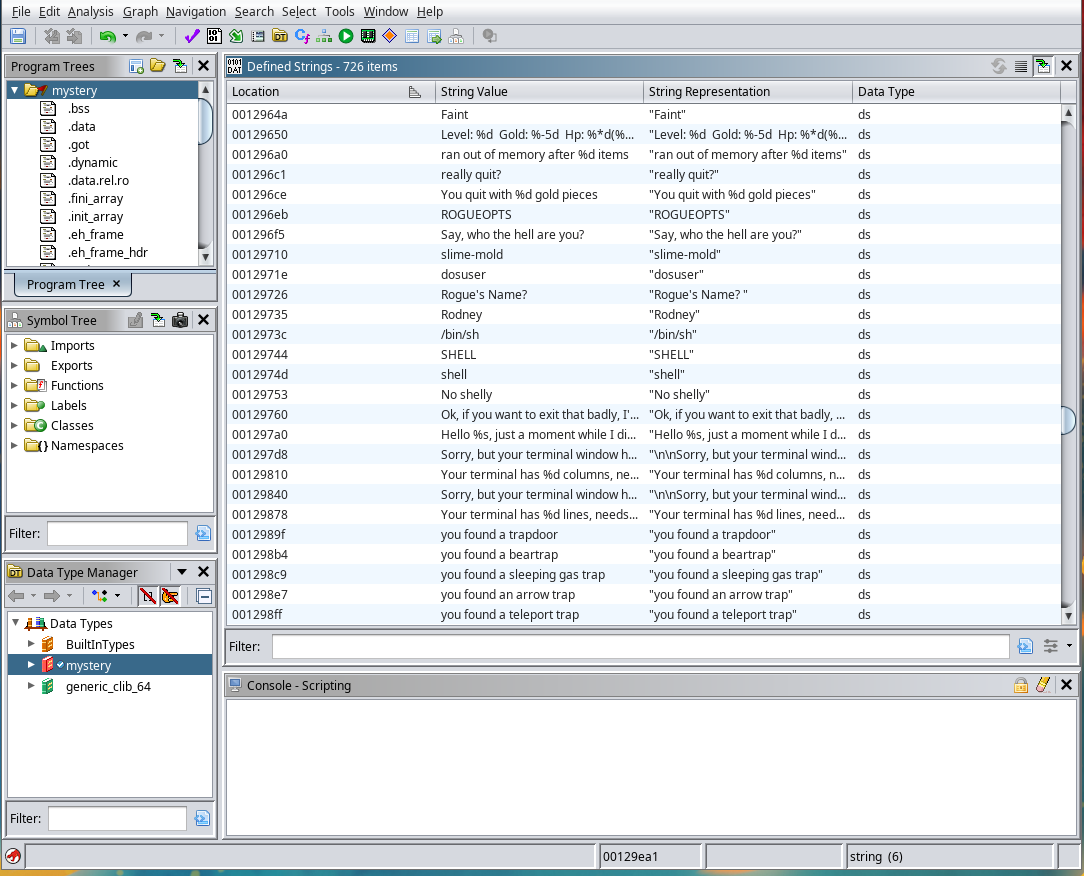
\includegraphics[width=0.8\textwidth]{../re-tools/ghidra-strings-mystery-ex}
\end{frame}



\section{finding library/system calls}

    % FIXME: objdump -R
    % FIXME: objdump -t

\begin{frame}[fragile]{libraries}
\begin{Verbatim}[fontsize=\small]
$ objdump --all-headers mystery
\end{Verbatim}
\ldots
\begin{Verbatim}[fontsize=\small]
Dynamic Section:
  NEEDED               libncurses.so.6
  NEEDED               libtinfo.so.6
  NEEDED               libc.so.6
\end{Verbatim}
\ldots
\end{frame}

\begin{frame}[fragile]{ncurses?}
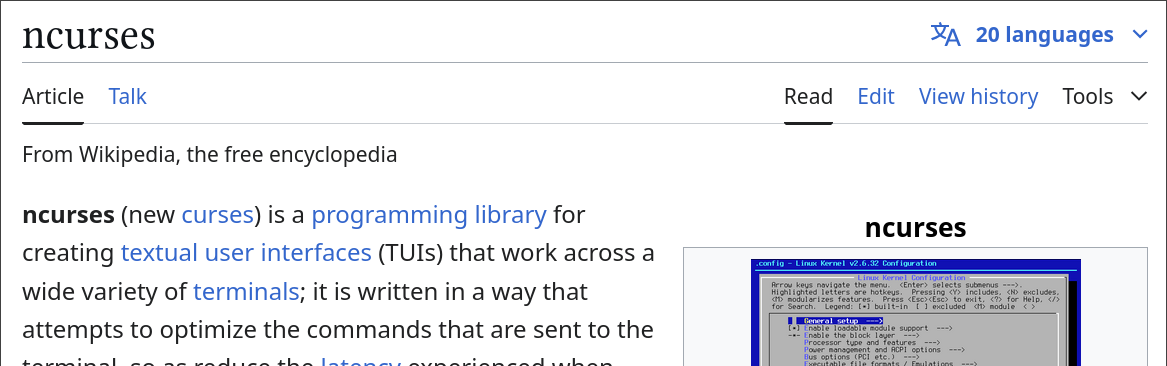
\includegraphics[width=\textwidth]{../re-tools/ncurses-wiki}
\end{frame}

\begin{frame}[fragile]{tinfo? (1)}
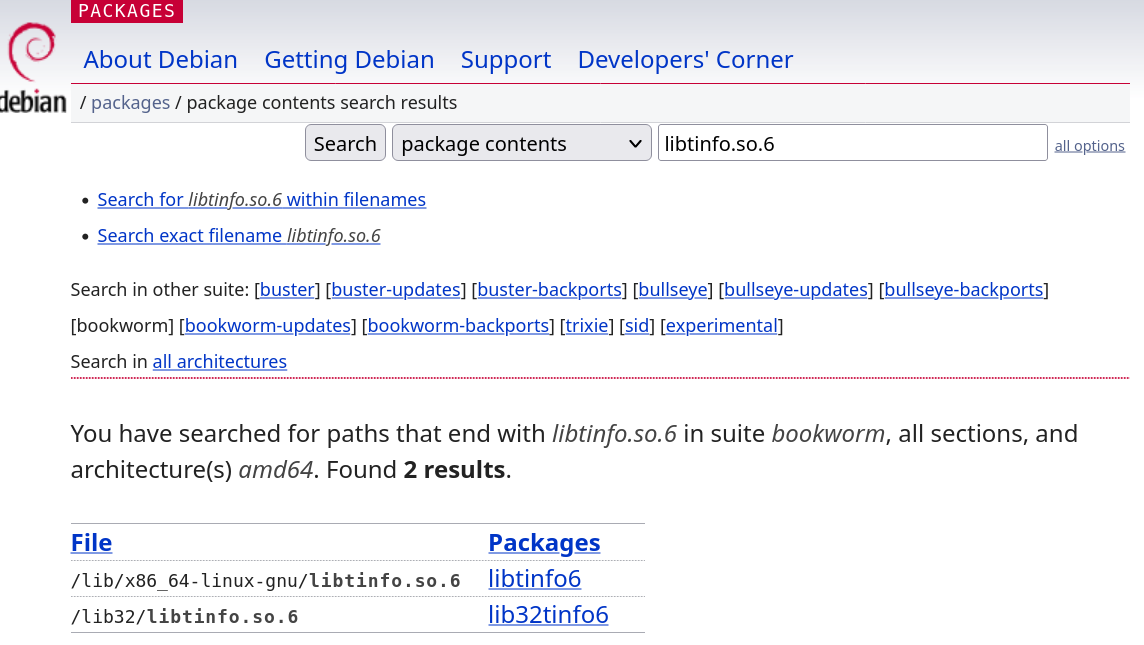
\includegraphics[width=0.7\textwidth]{../re-tools/deb-tinfo1}
\end{frame}

\begin{frame}[fragile]{tinfo? (2)}
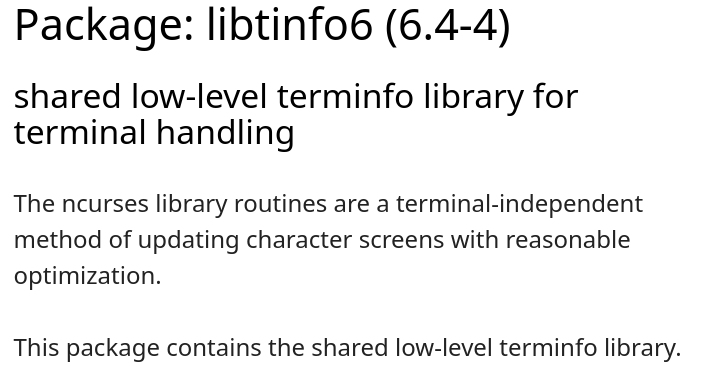
\includegraphics[width=0.7\textwidth]{../re-tools/deb-tinfo2}
\end{frame}

\begin{frame}[fragile]{library calls}
\begin{Verbatim}[fontsize=\fontsize{8}{9}]
$ objdump --dynamic-syms mystery

mystery:     file format elf64-x86-64

DYNAMIC SYMBOL TABLE:
0000000000000000      DF *UND*  0000000000000000 (GLIBC_2.3)  __ctype_toupper_loc
0000000000000000      DF *UND*  0000000000000000 (GLIBC_2.2.5) getenv
0000000000000000      DF *UND*  0000000000000000 (NCURSES6_5.0.19991023) wattrset
0000000000000000      DF *UND*  0000000000000000 (GLIBC_2.2.5) free
0000000000000000      DF *UND*  0000000000000000 (NCURSES6_TINFO_5.0.19991023) flushinp
0000000000000000      DF *UND*  0000000000000000 (GLIBC_2.2.5) localtime
0000000000000000      DF *UND*  0000000000000000 (GLIBC_2.34) __libc_start_main
\end{Verbatim}
\ldots
\begin{Verbatim}[fontsize=\fontsize{9}{10}]
0000000000000000      DF *UND*  0000000000000000 (GLIBC_2.2.5) setuid
\end{Verbatim}
\ldots
\end{frame}

\begin{frame}[fragile]{library calls (Ghidra)}
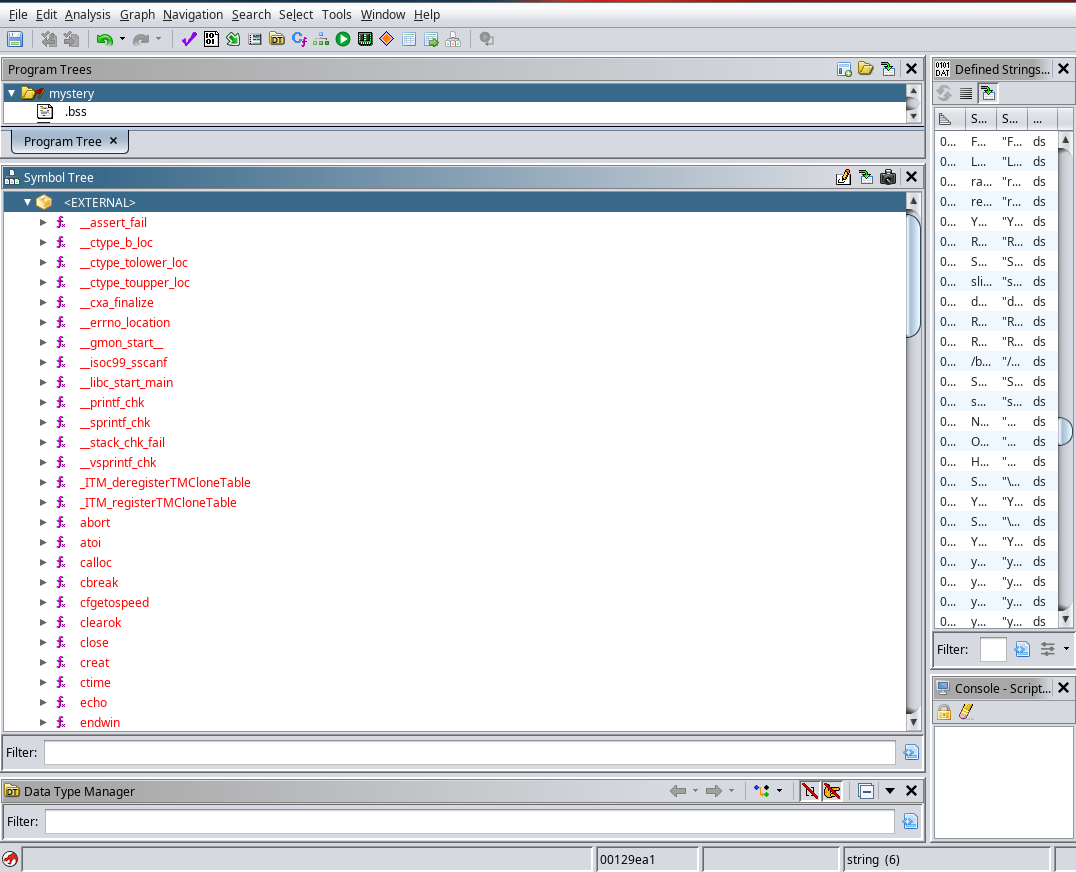
\includegraphics[width=\textwidth]{../re-tools/ghidra-mystery-ext}
\end{frame}

\begin{frame}[fragile]{finding library call uses}
{\small {\tt objdump --disassemble --dyanmic-reloc:}}
\begin{Verbatim}[fontsize=\fontsize{9}{10}]
0000000000005b00 <setuid@plt>:
    5b00:▶      f3 0f 1e fa          ▶  endbr64␣
    5b04:▶      f2 ff 25 fd d3 02 00 ▶  bnd jmp *0x2d3fd(%rip) 
			# 32f08 <setuid@GLIBC_2.2.5>
    5b0b:▶      0f 1f 44 00 00       ▶  nopl   0x0(%rax,%rax,1)
\end{Verbatim}
\ldots
\begin{Verbatim}[fontsize=\fontsize{9}{10}]
   2764f:▶      e8 ec e3 fd ff       ▶  call   5a40 <open@plt>
   27654:▶      89 05 fe 48 01 00    ▶  mov    %eax,0x148fe(%rip)        # 3bf58 <LINES@NCURSES6_TINFO_5.0.19991023+0x5244>
   2765a:▶      31 c0                ▶  xor    %eax,%eax
   2765c:▶      e8 2f e1 fd ff       ▶  call   5790 <getuid@plt>
   27661:▶      89 c7                ▶  mov    %eax,%edi
   27663:▶      31 c0                ▶  xor    %eax,%eax
   27665:▶      e8 96 e4 fd ff       ▶  call   5b00 <setuid@plt>
   2766a:▶      31 c0                ▶  xor    %eax,%eax
   2766c:▶      e8 cf e2 fd ff       ▶  call   5940 <getgid@plt>
   27671:▶      48 83 c4 08          ▶  add    $0x8,%rsp
\end{Verbatim}
\end{frame}

% FIXME: library call uses Ghidra


\section{disassembly, need for xrefs}
\begin{frame}[fragile]{disassembly issues (1)}
\begin{lstlisting}[language=myasm,style=size8]
.global main
main:
    call print_hello
    xorl %eax, %eax
    ret
.Lstr:
    .asciz "Hello!"
print_hello:
    leaq .Lstr(%rip), %rdi  // RDI <- .Lstr address
    jmp puts
\end{lstlisting}
\hrule
\begin{Verbatim}[fontsize=\fontsize{8}{9},commandchars=\\\{\}]
0000000000001139 <main>:
    1139:	e8 0a 00 00 00       	call   1148 <print_hello>
    113e:	31 c0                	xor    %eax,%eax
    1140:	c3                   	ret    
    \myemph{1141:	48                   	rex.W}
    \myemph{1142:	65 6c                	gs insb (%dx),%es:(%rdi)}
    \myemph{1144:	6c                   	insb   (%dx),%es:(%rdi)}
    \myemph{1145:	6f                   	outsl  %ds:(%rsi),(%dx)}
    \myemph{1146:	2e                   	cs}
\myemph{	...}
0000000000001148 <print_hello>:
    1148:	48 8d 3d f2 ff ff ff 	lea    -0xe(%rip),%rdi        # 1141 <main+0x8>
    114f:	e9 dc fe ff ff       	jmp    1030 <puts@plt>
\end{Verbatim}
\end{frame}

\begin{frame}[fragile]{disassembly issues}
\begin{Verbatim}[fontsize=\fontsize{8}{9},commandchars=\\\{\}]
0000000000001139 <main>:
    1139:	e8 0a 00 00 00       	call   1148 <print_hello>
    113e:	31 c0                	xor    %eax,%eax
    1140:	c3                   	ret    
    \myemph{1141:	48                   	rex.W}
    \myemph{1142:	65 6c                	gs insb (%dx),%es:(%rdi)}
    \myemph{1144:	6c                   	insb   (%dx),%es:(%rdi)}
    \myemph{1145:	6f                   	outsl  %ds:(%rsi),(%dx)}
    \myemph{1146:	2e                   	cs}
    \myemph{	...}
0000000000001148 <print_hello>:
    1148:	48 8d 3d f2 ff ff ff 	lea    -0xe(%rip),%rdi        # 1141 <main+0x8>
    114f:	e9 dc fe ff ff       	jmp    1030 <puts@plt>
\end{Verbatim}
\hrule
\begin{Verbatim}[fontsize=\fontsize{8}{9},commandchars=\\\{\}]
    1139:	e8 0a 00 00 00       	call   1148 <__cxa_finalize@plt+0x108>
    113e:	31 c0                	xor    %eax,%eax
    1140:	c3                   	ret    
    \myemph{1141:	48                   	rex.W}
    \myemph{1142:	65 6c                	gs insb (%dx),%es:(%rdi)}
    \myemph{1144:	6c                   	insb   (%dx),%es:(%rdi)}
    \myemph{1145:	6f                   	outsl  %ds:(%rsi),(%dx)}
    1146:	\myemph{2e 00} 48 8d          	cs add %cl,-0x73(%rax)
    114a:	3d f2 ff ff ff       	cmp    $0xfffffff2,%eax
    114f:	e9 dc fe ff ff       	jmp    1030 <puts@plt>
\end{Verbatim}
\end{frame}

\begin{frame}{finding assembly heuristics}
    \begin{itemize}
    \item objdump strategy, apparently:
        \begin{itemize}
        \item disassemble instructions starting at each symbol
        \item skip over strings of zero-bytes just before symbol
        \end{itemize}
    \item problem: can misidentify jumped to instructions
        \begin{itemize}
        \item especially if symbols stripped to save space/hinder reverse engineering
        \end{itemize}
    \item exercise: algorithm to fix?
        \begin{itemize}
        \item (Ghidra does this)
        \end{itemize}
    \end{itemize}
\end{frame}

% FIXME: exercise: Q: what to do about range of addresses given context?


\begin{frame}
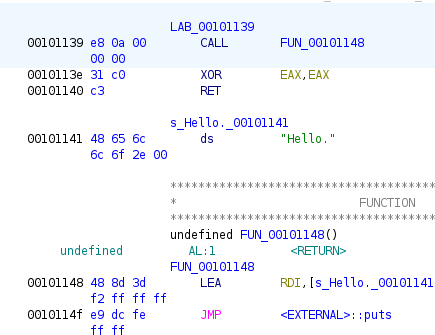
\includegraphics[width=\textwidth]{ghidra-disass-mixed-detail}
\end{frame}


\section{cross-references}
\begin{frame}{cross-references (1)}
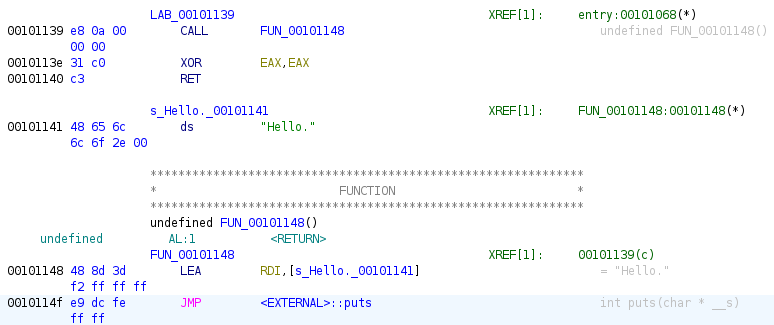
\includegraphics[width=\textwidth]{../re-tools/ghidra-disass-mixed-w-xref}
\end{frame}

\begin{frame}{cross-references idea}
    \begin{itemize}
    \item cross-reference idea:
    \item really useful to know where something is used
    \vspace{.5cm}
    \item do-able `by hand' with objdump and friends, but\ldots
        \begin{itemize}
        \item lots of bookkeeping, searching in text files, etc.
        \end{itemize}
    \end{itemize}
\end{frame}

\begin{frame}{more cross-references}
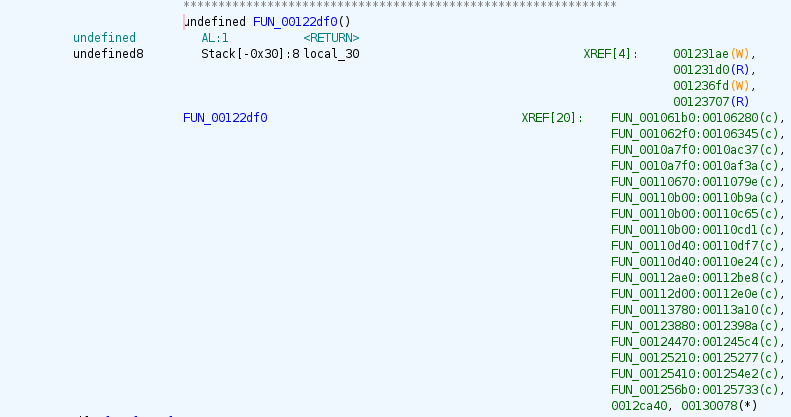
\includegraphics[width=\textwidth]{../re-tools/ghidra-mystery-xref-many}
\end{frame}




\section{high-level overviews}

\subsection{function callers/callees}
\begin{frame}{function callers?}
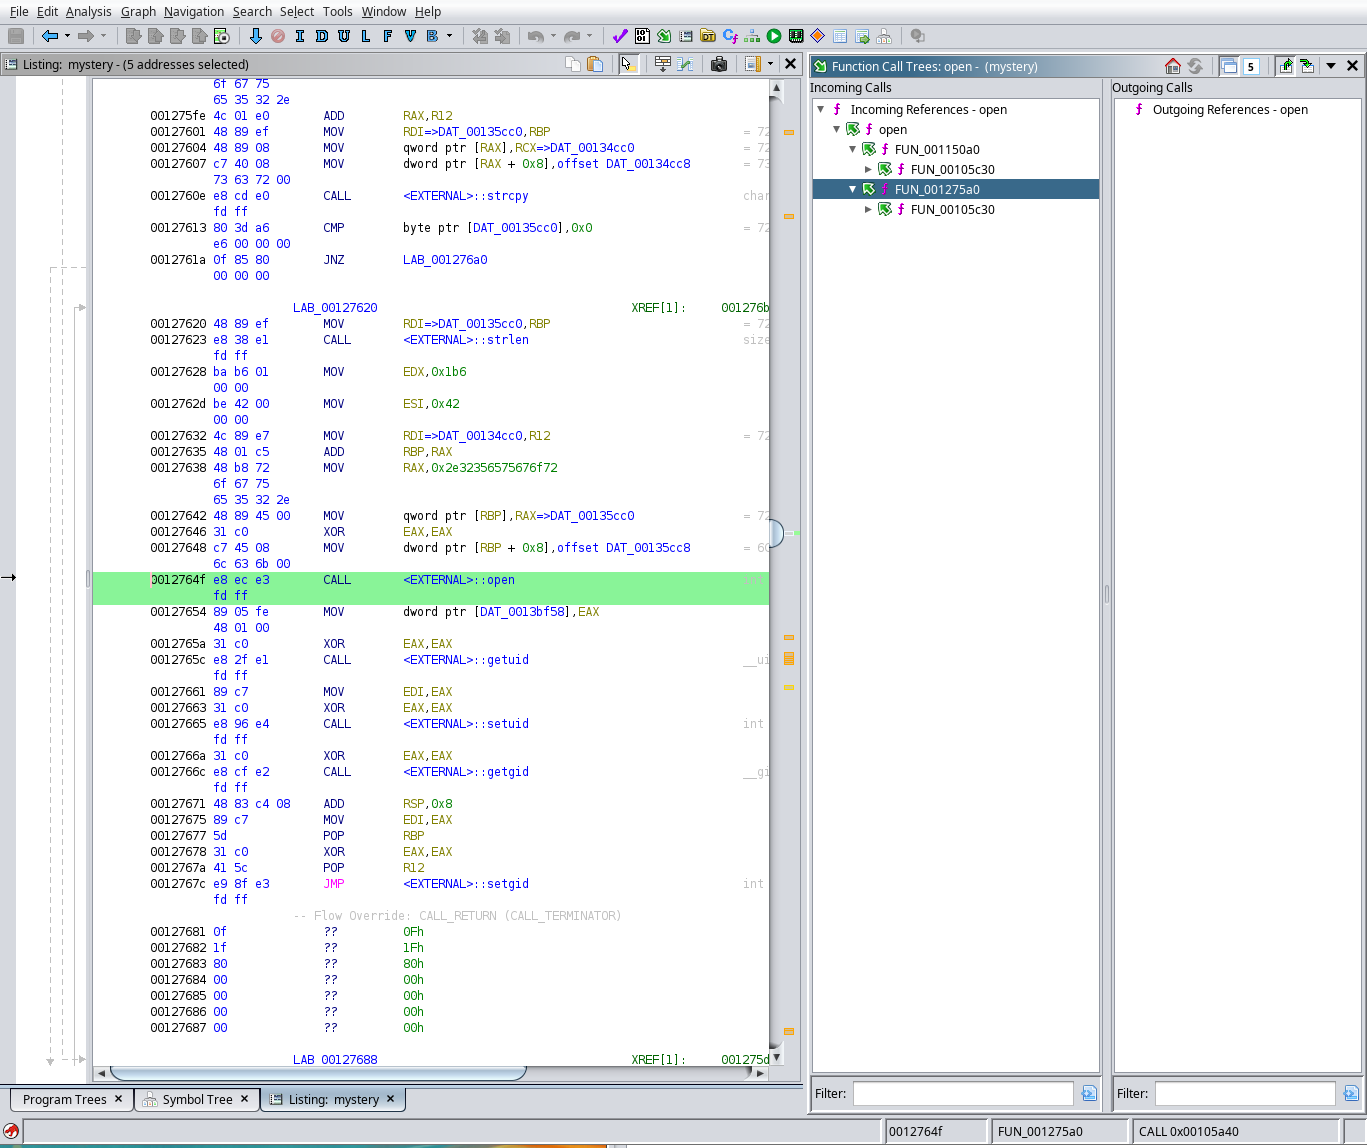
\includegraphics[width=\textwidth]{../re-tools/ghidra-symb-refs-ex}
\end{frame}

\begin{frame}{FUN\_12345678}
    \begin{itemize}
    \item Ghidra names functions without symbols based on address
    \item we can adjust that\ldots
    \end{itemize}
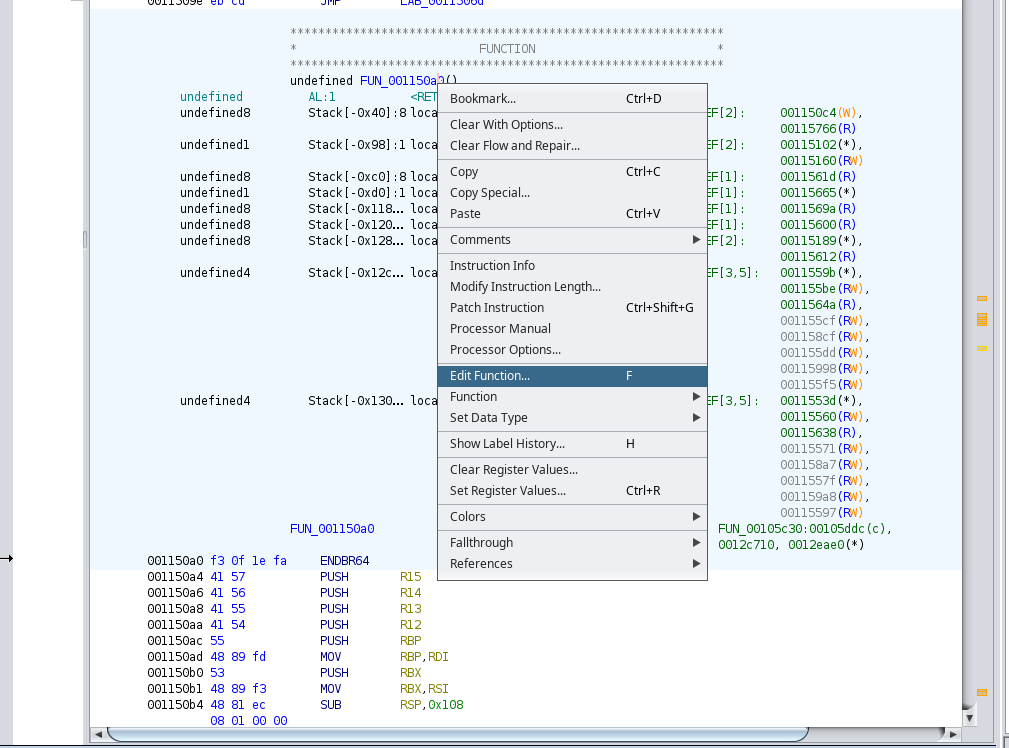
\includegraphics[width=0.45\textwidth]{../re-tools/ghidra-edit-func-cut}
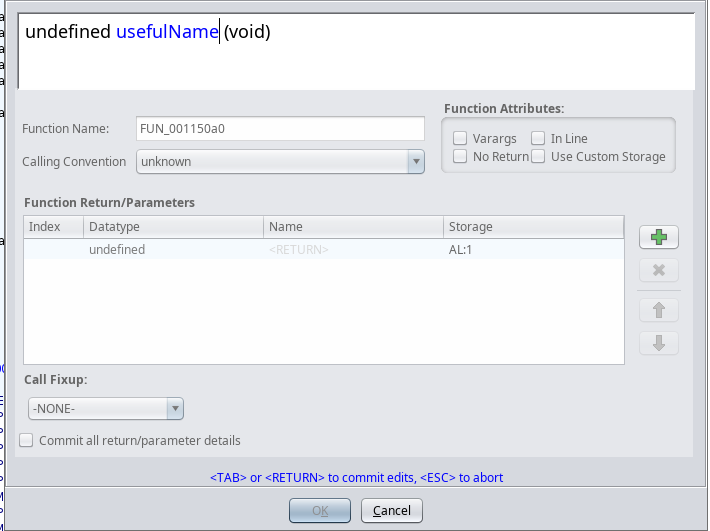
\includegraphics[width=0.45\textwidth]{../re-tools/ghidra-edit-func-dialog}
\end{frame}

 % FIXME: cleanup exercise

\subsection{control flow graphs}
\begin{frame}{}
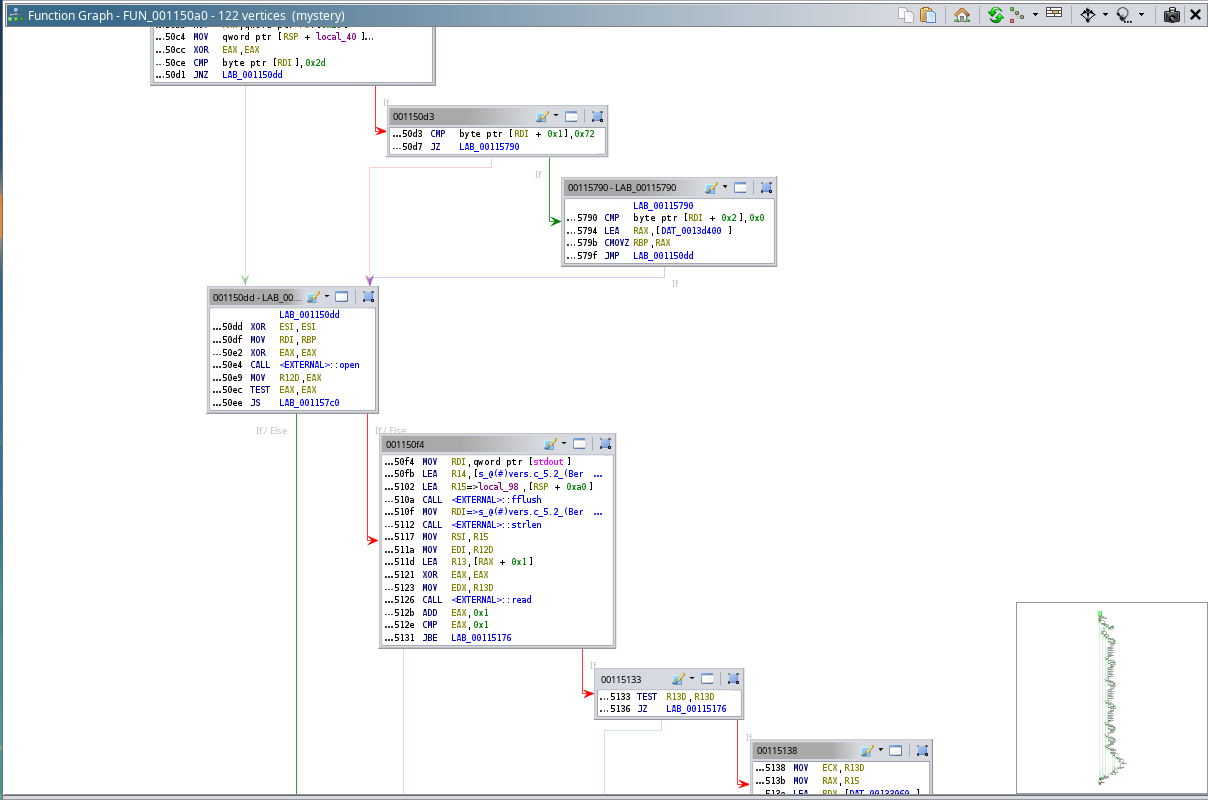
\includegraphics[height=0.95\textheight]{../re-tools/fun-graph-ex}
\end{frame}


\subsection{arrows on the side}
\begin{frame}{}
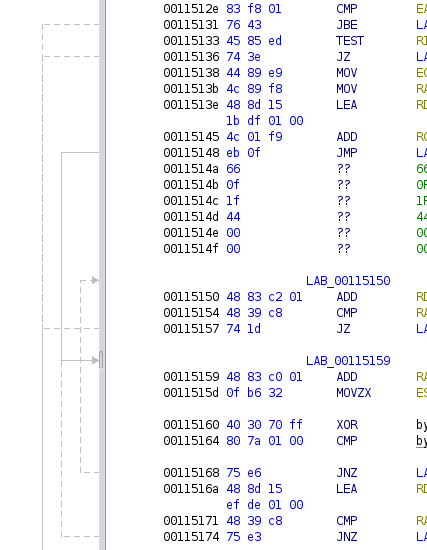
\includegraphics[height=0.9\textheight]{../re-tools/ghidra-side-arrows}
\end{frame}


\section{decompiling}

\subsection{decompiler}
\begin{frame}{decompiler}
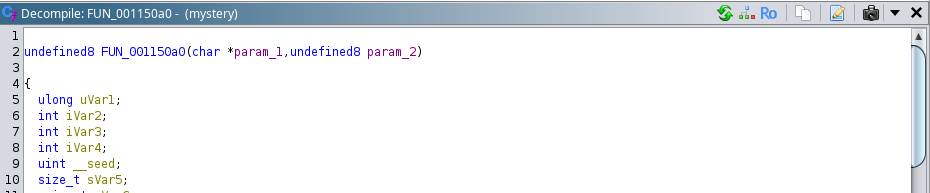
\includegraphics[width=0.9\textwidth]{../re-tools/decomp-top} \\
\ldots  \\
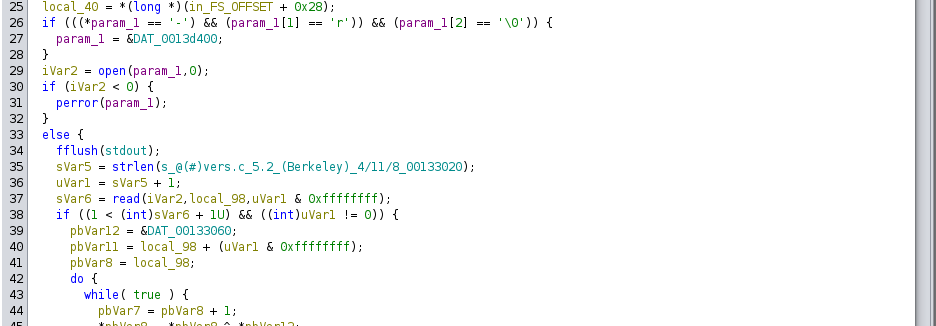
\includegraphics[width=0.9\textwidth]{../re-tools/decomp-rest}
\end{frame}

\begin{frame}{refining decompile (1)}
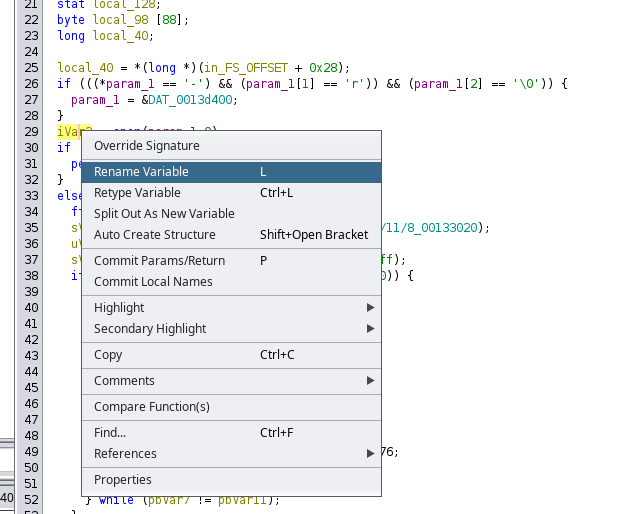
\includegraphics[width=0.9\textwidth]{../re-tools/ghidra-edit-var-decomp}
\end{frame}

\begin{frame}{refining decompile (2)}
    \begin{itemize}
    \item can setup names, types for functions
    \item types can include marking array
        \begin{itemize}
        \item Ghidra doesn't seem great at inferring this all the time
        \end{itemize}
    \vspace{.5cm}
    \item also for local/global variables
        \begin{itemize}
        \item for globals, can right-click in listing view too
        \end{itemize}
    \end{itemize}
\end{frame}



% intermediate representation for main() function in mystery
% decompiled representation
\subsection{Ghidra: intermediate representation}
\begin{frame}{interlude: editing disassembly format}
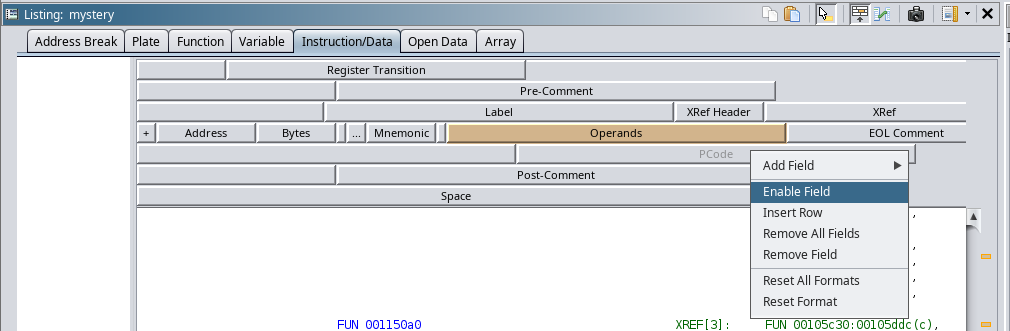
\includegraphics[width=\textwidth]{../re-tools/ghidra-enable-show-pcode}
\end{frame}

\begin{frame}{PCode}
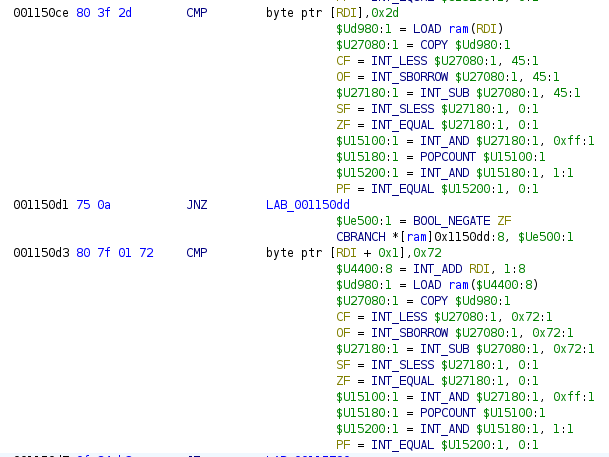
\includegraphics[height=0.9\textheight]{../re-tools/ghidra-pcode-ex}
\end{frame}

\begin{frame}{Intermediate Representations}
\begin{itemize}
\item Ghidra converts instructions to this PCode language
    \begin{itemize}
    \item describes effects of each instruction for other parts of Ghidra
    \item allows `easy' support for ARM, MIPS, \ldots
    \end{itemize}
\item function graph we saw using PCode information, probably
\item decompiler is basically a PCode to C compiler
    \begin{itemize}
    \item does the same kind of optimizations/etc. normal compiler does
    \item different output language
    \end{itemize}
\item Ghidra has `find similar functions' tool that probably uses this
\end{itemize}
\end{frame}




\section{more high-level overviews}

\subsection{data flow graphs}

\subsection{data type inference}

\section{annotate to improve}

\subsection{function naming}

\subsection{data, parameter types, arrays}

\section{patching things}
\begin{frame}{patch instruction?}
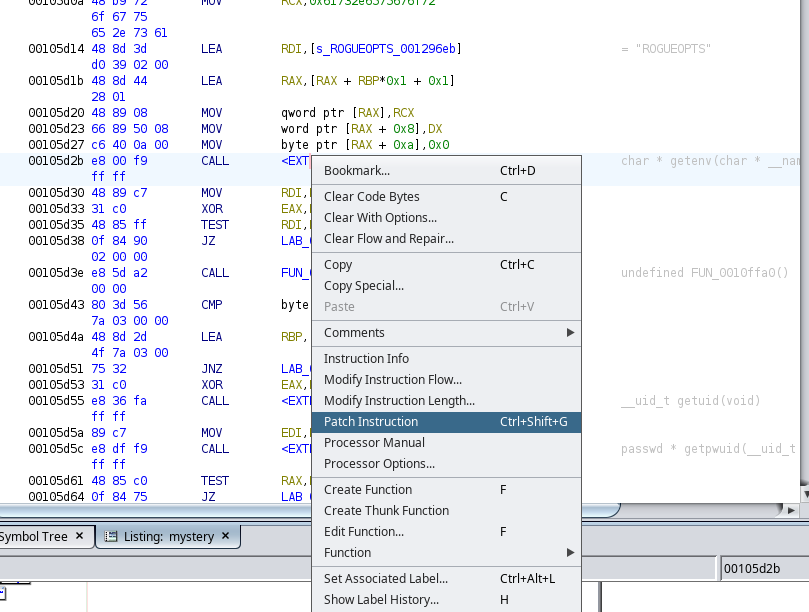
\includegraphics[width=\textwidth]{../re-tools/ghidra-patch-ex}
\end{frame}

\begin{frame}{patch instruction?}
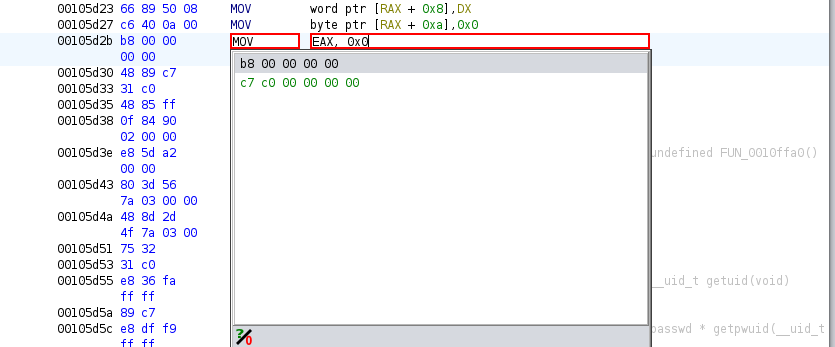
\includegraphics[width=\textwidth]{../re-tools/ghidra-patch-ex2}
\end{frame}

\begin{frame}{why is this useful?}
    \begin{itemize}
    \item can export modified version of binary to test
    \item ghidra has support for debugging or emulating running program
        \begin{itemize}
        \item emulation is another application of PCode representation
        \item debugging requires some work to configure
        \end{itemize}
    \end{itemize}
\end{frame}



\section{with debuggers}






\section{self-replicating malware, generally}

\usetikzlibrary{calc}

\begin{frame}{self-replicating malware}
    \begin{itemize}
    \item attacker's problem: \\getting malware to \myemph{run where they want}
    \item some options:
    \vspace{.5cm}
    \item connect to machine and install it there
    \item send to someone
    \item convince someone else to send it to someone
    \end{itemize}
    \begin{tikzpicture}[overlay,remember picture]
        \begin{visibleenv}<2>
        \node[draw,red!80!black,thick] at ([yshift=1cm]current page.south) {
            \large all automatable!
        };
        \end{visibleenv}
    \end{tikzpicture}
\end{frame}

\begin{frame}<1>{recall: kinds of malware}
    \begin{itemize}
    \item viruses --- infects \myemph{other programs}
    \item \myemph<3>{worms} --- own malicious programs
    \item \myemph<4>{trojans} --- useful (looking) program that also is malicious
    \item \myemph<2>{rootkit} --- silent control of system
    \end{itemize}
    \begin{tikzpicture}[overlay,remember picture]
        \begin{visibleenv}<2>
        \node[draw,red!80!black,thick] at ([yshift=1cm]current page.south) {
            only useful after compromising
        };
        \end{visibleenv}
        \begin{visibleenv}<3>
        \node[draw,red!80!black,thick,align=left] at ([yshift=1cm]current page.south) {
            needs to way to be run in the first place
        };
        \end{visibleenv}
        \begin{visibleenv}<3>
        \node[draw,red!80!black,thick] at ([yshift=1cm]current page.south) {
            targeted ``social engineering''
        };
        \end{visibleenv}
    \end{tikzpicture}
\end{frame}



% FIXME: aside on non-self-replicating malware issues coming up
    % stealth
    % detection

\section{virus: hide in existing programs}

\subsection{motivation}

\begin{frame}{viruses: hiding in files}
    \begin{itemize}
    \item get someone run your malware?
    \item program \myemph{they already want to run}
    \vspace{.5cm}
    \item to spread your malware?
    \item program \myemph<1-2>{they already want to copy}
    \vspace{.5cm}
    \item trojan approach: create/modify new program
    \item simpler: modify already used/shared program
    \end{itemize}
\end{frame}

\begin{frame}{viruses: infecting programs?}
    \begin{itemize}
    \item viruses infecting other programs seems less common
        \begin{itemize}
        \item (but hard to get good statistics\ldots)
        \end{itemize}
    \vspace{.5cm}
    \item but producing infected versions of legitimate software is common
        \begin{itemize}
        \item e.g. fake download site
        \end{itemize}
    \item techniques for automated infection similar to manual infection
    \end{itemize}
\end{frame}


\subsection{early prevalance/motivations}

\begin{frame}[fragile,label=commercial]{virus prevalence}
    \begin{itemize}
        \item viruses \myemph{on commerically sold software media}
        \item from 1990 memo by Chris McDonald:
\begin{Verbatim}[fontsize=\fontsize{8}{9}\selectfont]
4.  MS-DOS INFECTIONS

SOFTWARE                REPORTING LOCATION      DATE     VIRAL INFECTION

a.  Unlock Masterkey    Kennedy Space Center    Oct 89   Vienna
b.  SARGON III          Iceland                 Sep 89   Cascade (1704)
c.  ASYST RTDEMO02.EXE  Fort Belvoir            Aug 89   Jerusalem-B
d.  Desktop Fractal     Various                 Jan 90   Jerusalem (1813)
	Design System
e.  Bureau of the       Government Printing     Jan 90   Jerusalem-B
    Census, Elec. County   Office/US Census Bureau
    & City Data Bk., 1988
f.  Northern Computers  Iceland                 Mar 90   Disk Killer
    (PC Manufacturer shipped infected systems.)
5.  MACINTOSH INFECTIONS

    SOFTWARE            REPORTING LOCATION      DATE     VIRAL INFECTION

a.  NoteWriter          Colgate College         Sep 89   Scores and nVIR
.......
\end{Verbatim}
    \end{itemize}
\imagecredit{https://groups.google.com/forum/\#!original/comp.virus/XJCfYR9T6nI/azflHz5goooJ}
\end{frame}


\begin{frame}{early virus motivations}
    \begin{itemize}
        \item lots of (but not all) early virus software was ``for fun''
        \item not trying to monetize malware
            \begin{itemize}
            \item (like is common today)
            \end{itemize}
        \item hard: Internet connections uncommon
    \end{itemize}
\end{frame}





% FIXME: later prevalence

\section{case study: Vienna}

\begin{frame}{Case Study: Vienna Virus}
\begin{itemize}
    \item Vienna: virus from the 1980s
    \item This version: published in Ralf Burger, ``Computer Viruses: a high-tech disease'' (1988)
    \item targetted COM-format executables on DOS
\end{itemize}
\end{frame}




\subsection{aside: COM files}


\begin{frame}{Diversion: .COM files}
    \begin{itemize}
    \item .COM is a \myemph{very simple} executable format
    \item no header, no segments, no sections
    \item file contents loaded at fixed address {\tt 0x0100}
    \item execution starts at {\tt 0x0100}
    \item everything is read/write/execute (no virtual memory)
    \end{itemize}
\end{frame}




\subsection{entry/exit}

\usetikzlibrary{calc}

\begin{frame}[fragile,label=vienna]{Vienna: infection}
\lstset{
    language=myasm,
    style=smaller,
    moredelim={**[is][\btHL<2>]{~hi2~}{~endhi2~}},
}
\begin{tikzpicture}
\tikzset{programBox/.style={draw,thick},every label/.style={inner sep=1mm,outer sep=0mm}}
\node[programBox,minimum height=3cm,label={north:uninfected},anchor=north west] (uninfect) at (0,0) {
\begin{lstlisting}
0x0100:
    ~hi2~mov $0x4f28, %cx~endhi2~
    /* b9 28 4f */
0x0103:
    mov $0x9e4e, %si
    /* be 4e 9e */
    mov %si, %di
    push %ds
    /* more normal
       program
       code */
....
0x0700: /* end */

\end{lstlisting}
};
\node[overlay,programBox,anchor=north west,label={[overlay]north:infected}] at ([yshift=.5cm,xshift=1cm]uninfect.north east) {
\begin{lstlisting}
0x0100: jmp 0x0700
0x0103: mov $0x9e4e, %si
...
0x0700:
    push %cx
    ... // %si <- 0x903
    mov $0x100, %di
    mov $3, %cx
    rep movsb
    ...
    mov $0x0100, %di
    push %di
    xor %di, %di
    ret
...
0x0903:
    ~hi2~.bytes 0xb9 0x28 0x4f~endhi2~
...
\end{lstlisting}
};
\end{tikzpicture}
\end{frame}

\begin{frame}[fragile,label=viennaFixup]{Vienna: ``fixup''}
\lstset{
    language=myasm,
    style=small,
    moredelim={**[is][\btHL<2>]{~hi2~}{~endhi2~}},
    moredelim={**[is][\btHL<3>]{~hi3~}{~endhi3~}},
}
\begin{lstlisting}
0x0700:
    push %cx // initial value of %cx matters??
    mov ~hi3~$0x8fd~endhi3~, %si // %si <- beginning of data
    mov %si, %dx // save %si
        // movsb uses %si, so
        // can't use another register
    add $0xa, %si // offset of saved code in data
    mov $0x100, %di // target address
    mov $3, %cx // bytes changed
    /* copy %cx bytes from (%si) to (%di) */
    rep movsb 
    ...
...
// saved copy of original application code
0x903: ~hi2~.byte 0xb9 .byte 0x28 .byte 0x4f~endhi2~
\end{lstlisting}
\end{frame}

\begin{frame}[fragile,label=viennaReturn]{Vienna: return}
\lstset{language=myasm,style=small}
\begin{lstlisting}
0x08e7:
    pop %cx // restore initial value of %cx, %sp
    xor %ax, %ax // %ax <- 0
    xor %bx, %bx
    xor %dx, %dx
    xor %si, %si
    // push 0x0100
    mov $0x0100, %di
    push %di 
    xor %di, %di // %di <- 0
    // pop 0x0100 from stack
    // jmp to 0x0100
    ret 
\end{lstlisting}
\begin{itemize}
\item<1> question: why not just jmp 0x0100 ?
\end{itemize}
\end{frame}



\subsection{infection outline}


\begin{frame}<1>[label=viennaOutline]{Vienna: infection outline}
\begin{itemize}
\item Vienna \myemph{appends} code to infected application
\vspace{.5cm}
\item \myemph<2>{where does it read the code come from?}
\item \myemph<3>{how is code adjusted for new location in the binary?}
    \begin{itemize}\item what linker would do\end{itemize}
\item \myemph<4>{how does it keep files from getting infinitely long?}
\end{itemize}
\end{frame}


\subsection{writing your own code?}

\againframe<2>{viennaOutline}
\subsubsection{aside: quines}


\begin{frame}{quines}
\begin{itemize}
    \item exercise: write a C program that outputs its source code
        \begin{itemize}
        \item (pseudo-code only okay)
        \end{itemize}
    \item possible in any {\small (Turing-complete)} programming language
    \item called a ``quine''
\end{itemize}
\end{frame}

\begin{frame}[fragile,label=quineClever]{clever quine solution}
\lstset{language=C,style=small,
    moredelim={**[is][\btHL<2|handout:0>]{@hi2@}{@endhi@}},
    moredelim={**[is][\btHL<3|handout:0>]{@hi3@}{@endhi@}},
    showstringspaces=false,
}
\begin{lstlisting}
#include <stdio.h>
char*x="int main(){
       `\btHL<2>{printf(p,10,34,x,34,10,34,p,34,10,x,10);}`
       }";
@hi3@char*p@endhi@="#include <stdio.h>%c
    char*x=%c%s%c;%cchar*p=%c%s%c;
    %c%s%c";
int main(){
    @hi2@printf(p,10,34,x,34,10,34,p,34,10,x,10);@endhi@
}
\end{lstlisting}
\begin{itemize}
\item some line wrapping for readability --- shouldn't be in actual quine
\end{itemize}
\begin{tikzpicture}[overlay,remember picture]
    \begin{visibleenv}<2|handout:0>
        \node[fill=white,draw,thick,align=left] at (current page.center) {
            {\tt printf} to fill template: \\
            {\tt 10} = newline; {\tt 34} = double-quote; \\
            {\tt x}, {\tt p} = template/constant strings
        };
    \end{visibleenv}
    \begin{visibleenv}<3|handout:0>
        \node[fill=white,draw,thick,align=left] at ([yshift=1cm]current page.center) {
            template filled by printf
        };
    \end{visibleenv}
\end{tikzpicture}
\end{frame}

\begin{frame}[fragile,label=quineDumb]{dumb quine solution}
\begin{lstlisting}[language=C,style=small]
#include <stdio.h>
int main(void) {
    char buffer[1024];
    FILE *f = fopen("quine.c", "r");
    size_t bytes = fread(buffer, 1,
                         sizeof(buffer), f);
    fwrite(buffer, 1, bytes, stdout);
    return 0;
}
\end{lstlisting}
\begin{itemize}
\item a lot more straightforward!
\item but ``cheating''
\end{itemize}
\end{frame}



\subsubsection{Vienna replication code}


\begin{frame}[fragile,label=virusWriting]{Vienna copying}
\lstset{
    style=small,
    language=myasm,
    moredelim={**[is][\btHL<2|handout:0>]{@hi2@}{@endhi@}},
}
\begin{lstlisting}
@hi2@mov $0x8f9, %si@endhi@ // %si = beginning of virus data
...
mov $0x288, %cx // length of virus
mov $0x40, %ah  // system call # for write
mov %si, %dx
sub $0x1f9, %dx // %dx = beginning of virus code
int 0x21 // make write system call
\end{lstlisting}
\end{frame}




\subsection{Vienan relocation code}
% FIXME: need to explain why this is a problem
\againframe<3>{viennaOutline}

\subsubsection{Vienna's relocation code}

\begin{frame}[fragile,label=virusReloc2]{Vienna relocation}
\lstset{
    style=small,
    language=myasm,
    moredelim={**[is][\btHL<1|handout:0>]{@hi1@}{@endhi@}},
    moredelim={**[is][\btHL<2|handout:0>]{@hi2@}{@endhi@}},
    moredelim={**[is][\btHL<3|handout:0>]{@hi3@}{@endhi@}},
}
\begin{lstlisting}
// set virus data address:
0x700: @hi1@mov $0x8f9, %si@endhi@
       // machine code: be f9 08
       // be: opcode
       // f9 08: immediate
...
// %ax contains file length (of file to infect)
mov %ax, %cx
...
@hi3@add $0x2f9, %cx@endhi@
mov %si, %di   
sub $0x1f7, %di // %di <- 0x701
@hi2@mov %cx, (%di)@endhi@  // update mov instruction
...
\end{lstlisting}
\begin{tikzpicture}[overlay,remember picture]
\begin{visibleenv}<1>
\node[align=left,draw,very thick,fill=white] at (current page.center) {
    Vienna design: need to access global variables, etc. \\
    solution: base pointer for virus data \\
    problem: location changes depending on where virus is
};
\end{visibleenv}
\end{tikzpicture}
\end{frame}

\begin{frame}[fragile,label=virusReloc3]{Vienna relocation}
\begin{itemize}
\item edit actual code for {\tt mov}
\item why doesn't this disrupt virus execution?
    \begin{itemize}\item<2> already ran that instruction\end{itemize}
\end{itemize}
\end{frame}

\begin{frame}[fragile,label=virusReloc4]{Vienna relocation}
\lstset{
    style=smaller,
    language=myasm,
    moredelim={**[is][\btHL<2|handout:0>]{@hi2@}{@endhi@}},
    moredelim={**[is][\btHL<3|handout:0>]{@hi3@}{@endhi@}},
}
\begin{lstlisting}
0x700: mov $0x8f9, %si
...
// %ax contains file length
//     (of file to infect)
mov %ax, %cx
sub $3, %ax
// update template jmp instruction
mov %ax, @hi2@0xe(%si)@endhi@ // 0xe + %si = 0x907
...
mov $40, %ah
mov $3, %cx
mov %si, %dx  
add $0xD, @hi3@%dx@endhi@ // dx <- 0x906
int 0x21 // system call: write 3 bytes from 0x906
...
0x906: @hi2@e9 fd 05@endhi@ // jmp PC+FD 05
\end{lstlisting}
\end{frame}



\subsubsection{alternate: PIC}

\begin{frame}[fragile,label=altVirusReloc]{alternative relocation}
    \begin{itemize}
    \item could avoid having pointer to update:
    \end{itemize}
\begin{Verbatim}[fontsize=\fontsize{10}{11}\selectfont,commandchars=Q\{\}]
0000000000000000 <next-0x3>:
   0:   e8 Qtextbf{00 00}                call   3 <next>
    Qtextit{target addresses encoded relatively}
    Qtextit{pushes return address (next) onto stack}
0000000000000003 <next>:
   3:   59                      pop    %cx
    Qtextit{cx containts address of the pop instruction}
\end{Verbatim}
    \begin{itemize}
    \item why didn't Vienna do this?
    \end{itemize}
\end{frame}



\subsection{avoiding reinfection}
\againframe<4>{viennaOutline}

\begin{frame}{Vienna: avoiding reinfection}
\begin{itemize}
\item scans through active directories for executables
\item ``marks'' infected executables in \myemph{file metadata}
\begin{itemize}
    \item could have checked for virus code --- but slow
\end{itemize}
\end{itemize}
\end{frame}

\begin{frame}{DOS last-written times}
\begin{itemize}
    \item 16-bit number for date; 16-bit number for time
\end{itemize}
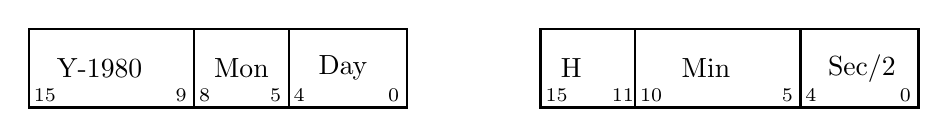
\begin{tikzpicture}
\tikzset{
    mylabel/.style={anchor=center},
    bitlabel/.style={font=\scriptsize,anchor=south west,inner sep=.5mm,text depth=.1mm},    
};
\begin{scope}[x=1.2cm]
\begin{scope}[thick]
    \draw (0, 0) rectangle (4, 1);
    \draw (0, 0) rectangle (1.75, 1);
    \node[bitlabel] at (0, 0) {15};
    \node[bitlabel] at (1.5, 0) {9};
    \draw (1.75, 0) rectangle (2.75, 1);
    \node[bitlabel] at (1.75, 0) {8};
    \node[bitlabel] at (2.5, 0) {5};
    \draw (2.75, 0) rectangle (4., 1);
    \node[bitlabel] at (2.75, 0) {4};
    \node[bitlabel] at (3.75, 0) {0};
\end{scope}
\node[mylabel] at (.75, 0.5) {Y-1980};
\node[mylabel] at (2.25, 0.5) {Mon};
\node[mylabel] at (3.325, 0.5) {Day};
\end{scope}

\begin{scope}[x=1.2cm,xshift=6.5cm]
\begin{scope}[thick]
    \draw (0, 0) rectangle (4, 1);
    \draw (0, 0) rectangle (1, 1);
    \node[bitlabel] at (0, 0) {15};
    \node[bitlabel] at (.7, 0) {11};
    \draw (1, 0) rectangle (2.75, 1);
    \node[bitlabel] at (1.0, 0) {10};
    \node[bitlabel] at (2.5, 0) {5};
    \draw (2.75, 0) rectangle (4., 1);
    \node[bitlabel] at (2.75, 0) {4};
    \node[bitlabel] at (3.75, 0) {0};
\end{scope}
\node[mylabel] at (.325, 0.5) {H};
\node[mylabel] at (1.75, 0.5) {Min};
\node[mylabel] at (3.4, 0.5) {Sec/2};
\end{scope}
\end{tikzpicture}
\begin{itemize}
    \item<2> Sec/2: 5 bits: range from 0--31
        \begin{itemize}
        \item corresponds to 0 to \textbf{62} seconds
        \end{itemize}
    \item<2> Vienna trick: set infected file times to \textbf{62} seconds
    \item<2> need to update times anyways --- hide tracks
\end{itemize}
\end{frame}



% FIXME: reflection on Vienna detection/portability
    % preview of future topics
        % looking for virus patterns that won't appear in executables

% FIXME: copy intro

\section{viruses: where to put code}


\begin{frame}{where to put code}
    \begin{itemize}
    \item viruses insert code in other programs
    \item Vienna's choice: end of executables
    \item search for \texttt{.COM} executables on system
    \vspace{.5cm}
    \item considerations for other options:
    \item spreading: identifying useful files to infect
        \begin{itemize}
        \item will be copied elsewhere?
        \item will be run?
        \end{itemize}
    \item stealth: avoiding detection
        \begin{itemize}
        \item Vienna: file size changes --- easy to find?
        \item Vienna: weird modification time --- easy to find?
        \end{itemize}
    \end{itemize}
\end{frame}

\begin{frame}<1>[label=whereCode]{where to put code: options}
    \begin{itemize}
    \item one \textit{or more} of:
    \item \myemph<2>{replacing executable code}
    \item \myemph<3>{after executable code (Vienna)}
    \item \myemph<4>{in unused executable code}
    \item \myemph<5>{inside OS code}
    \item \myemph<6>{in memory}
    \item \myemph<7>{replace existing code}
    \end{itemize}
\end{frame}



\subsection{replacing executables?}

\againframe<2>{whereCode}

\usetikzlibrary{arrows.meta}

\begin{frame}{replace executable}
    \begin{tikzpicture}
    \draw[thick] (0, 0) rectangle (4, -6) node[midway,align=center] {original\\executable};
    \draw[line width=2mm,-Latex,black!60] (4.1, -3) -- (6.9, -.5);
    \begin{scope}[xshift=7cm]
    \draw[thick,fill=red!20] (0, 0) rectangle (4, -1) node[midway,align=center] {virus code};
    \end{scope}
    \end{tikzpicture}
\end{frame}

\begin{frame}{replace executable?}
    \begin{itemize}
    \item seems silly --- not stealthy!
    \item has appeared in the wild --- ILOVEYOU
    \item 2000 ILOVEYOU Worm
        \begin{itemize}
        \item written in Visual Basic (!)
        \item spread via email
        \item replaced lots of files with copies of itself
        \end{itemize}
    \item huge impact --- because destroying data to copy itself
    \end{itemize}
\end{frame}

\begin{frame}{replace executable --- subtle}
    \begin{tikzpicture}
    \draw[thick] (0, 0) rectangle (4, -6) node[midway,align=center] {original\\executable};
    \draw[line width=2mm,-Latex,black!60] (4.1, -3) -- (6.9, -.5);
    \begin{scope}[xshift=7cm]
    \draw[thick,fill=red!20] (0, 0) rectangle (4, -1) node[midway,align=center] {virus code};
    \draw[thick,fill=yellow!20] (0, -1) rectangle (4, -1.5) node[midway,align=center,font=\scriptsize] {
        run original from tempfile
    };
    \draw[thick] (0, -1.5) rectangle (4, -7.2) node[midway,align=center] {original\\executable};
    \end{scope}
    \end{tikzpicture}
\end{frame}



\subsection{appending/compressing}

% FIXME: good place for aside on modern executable formats

\againframe<3>{whereCode}

\usetikzlibrary{arrows.meta,patterns}
\begin{frame}{appending}
    \pdftooltip{
    \begin{tikzpicture}
    \draw[thick] (0, 0) rectangle (4, -5) node[midway,align=center] {original\\executable};
    \draw[line width=2mm,-Latex,black!60] (4.1, -3) -- (6.9, -3);
    \begin{scope}[xshift=7cm]
    \draw[thick] (0, 0) rectangle (4, -5) node[midway,align=center] {original\\executable};
    \draw[fill=red!20,thick] (0, -5) rectangle (4, -6)
        node[midway,align=center] {virus code};
    \draw[fill=red!20,thick] (0.5, -1) rectangle (1, -1.5);
    \node[anchor=west,red!50!black] at (1.25, -1.25) {jmp to virus};
    \draw[thick,Latex-] (1, -1.25) -- (1.4, -1.25);
    \end{scope}
    \end{tikzpicture}
    }{executable transformed by replacing some of the original code with jmp + appending virus}
\end{frame}

\begin{frame}{appending and executable formats}
    \begin{itemize}
    \item COM files are very simple --- no metadata
    \item modern executable formats have length information to update:
    \vspace{.5cm}
    \item option 1: add segment (ELF LOAD) to program header
        \begin{itemize}
        \item (often a little extra space after program header, due to page-alignment)
        \end{itemize}
    \item option 2: update last segment of program header
        \begin{itemize}
        \item change its size
        \item make it executable if it isn't (and often not --- often data)
        \end{itemize}
    \end{itemize}
\end{frame}





\subsection{cavaties}

\againframe<4>{whereCode}

\begin{frame}{unused code???}
    \begin{itemize}
    \item why would a program have unused code????
    \end{itemize}
\end{frame}

\begin{frame}[fragile,label=lsStudy1]{unused code case study: /bin/ls}
    \begin{itemize}
    \item unreachable no-ops!
    \end{itemize}
\begin{Verbatim}[fontsize=\fontsize{9}{10}\selectfont,commandchars=Q\{\}]
...
  403788:	e9 59 0c 00 00       	jmpq   4043e6 <__sprintf_chk@plt+0x1a06>
  Qtextbf{40378d:	0f 1f 00             	nopl   (%rax)}
  403790:	ba 05 00 00 00       	mov    $0x5,%edx
...
  403ab9:	eb 4d                	jmp    403b08 <__sprintf_chk@plt+0x1128>
  Qtextbf{403abb:	0f 1f 44 00 00       	nopl   0x0(%rax,%rax,1)}
  403ac0:	4d 8b 7f 08          	mov    0x8(%r15),%r15
...
  404a01:	c3                   	retq   
  Qtextbf{404a02:	0f 1f 40 00          	nopl   0x0(%rax)}
  Qtextbf{404a06:	66 2e 0f 1f 84 00 00 	nopw   %cs:0x0(%rax,%rax,1)}
  Qtextbf{404a0d:	00 00 00 }
  404a10:	be 00 e6 61 00       	mov    $0x61e600,%esi
...
\end{Verbatim}
\end{frame}

\begin{frame}{why empty space?}
\begin{itemize}
\item Intel Optimization Reference Manual: \\
``\textbf{Assembly/Compiler Coding Rule 12. (M impact, H generality)} \\All branch targets should be 16-byte aligned.''
\vspace{.5cm}
    \item better for instruction cache {\small (and TLB and related caches)}
    \item better for instruction decode logic
    \item function calls, jumps count as branches for this purpose
\end{itemize}
\end{frame}

\begin{frame}{why weird nops}
    \begin{itemize}
    \item could fill with \myemph{anything} --- unreachable
    \item some platforms: filled with crashing instructions
    \vspace{.5cm}
    \item why not in example? assembler just told to align instruction
        \begin{itemize}
        \item not told previous instruction was jump/ret/etc. \ldots
        \item and assembler doesn't bother checking
        \end{itemize}
    \item probably better for CPU to fill with some instruction; Intel manual:
        \begin{itemize}
        \item ``Placing data immediately following an indirect branch
              can cause performance problems. If the data consists of all zeros,
              it looks like a long stream of ADDs to memory destinations, and this can cause
              resource conflicts\ldots''
        \end{itemize}
    \end{itemize}
\end{frame}

\begin{frame}<1>[label=otherSpace]{other empty space}
\begin{itemize}
\item \myemph<2>{unused dynamic linking structure}
\item \myemph<3>{unused space between segments}
\item unused debugging/symbol table information?
\item unused header space 
    \begin{itemize}
    \item file offsets of segments can be in middle of header
    \item loader doesn't care what segments ``mean''
    \end{itemize}
\end{itemize}
\end{frame}

\againframe<2>{otherSpace}

\begin{frame}[label=spaceDyn,fragile]{dynamic linking cavity}
\begin{itemize}
\item {\tt .dynamic} section --- data structure used by dynamic linker:
\item format: list of 8-byte type, 8-byte value
    \begin{itemize}
    \item terminated by type == 0 entry
    \end{itemize}
\end{itemize}
\begin{Verbatim}[fontsize=\fontsize{9}{10}\selectfont,commandchars=Q\{\}]
Contents of section .dynamic:
 600e28 01000000 00000000 01000000 00000000  ................
    Qtextit{... several non-empty entries ...}
 600f88 f0ffff6f 00000000 56034000 00000000  ...o....V.@.....
    Qtextit{VERSYM (required library version info at) 0x400356}
 600f98 Qtextit{00000000 00000000 00000000 00000000}  ................
    Qtextit{NULL --- end of linker info}
 600fa8 Qtextbf{00000000 00000000 00000000 00000000}  ................
    Qtextit{unused! (and below)}
 600fb8 Qtextbf{00000000 00000000 00000000 00000000}  ................
 600fc8 Qtextbf{00000000 00000000 00000000 00000000}  ................
 600fd8 Qtextbf{00000000 00000000 00000000 00000000}  ................
 600fe8 Qtextbf{00000000 00000000 00000000 00000000}  ................
\end{Verbatim}
\end{frame}





\subsubsection{chaining cavaties (CIH case study)}

\usetikzlibrary{arrows.meta,patterns}

\begin{frame}{is there enough empty space?}
\begin{itemize}
    \item cavities look awfully small
    \item really small viruses?
    \item solution: chain cavities tgoether
\end{itemize}
\end{frame}

\begin{frame}{case study: CIH (1)}
    \begin{tikzpicture}
    \draw[thick] (0, 0) rectangle (4, -6) node[midway,align=center] {original\\executable};
    \draw[line width=2mm,-Latex,black!60] (4.1, -3) -- (6.9, -3);
    \begin{scope}[xshift=7cm]
    \draw[fill=red!20,thick] (0, 0) rectangle (4, -0.5) node[midway] {virus startup code};
    \draw[fill=red!20,thick] (0, -0.5) rectangle (4, -1) node[midway] {virus code locs};
    \draw[thick] (0, -1) rectangle (4, -6);
    \draw[fill=red!20,thick] (0, -3) rectangle (4, -3.5)
        node[midway] {virus code part 1};
    \draw[fill=red!20,thick] (0, -4) rectangle (4, -4.5)
        node[midway] {virus code part 2};
    \draw[fill=red!20,thick] (0, -5) rectangle (4, -5.5)
        node[midway] {virus code part 3};
    \draw[dashed,thin,-Latex] (4, -0.75) -- (4.5, -0.75) |- (4, -3.25);
    \draw[dashed,thin,-Latex] (4, -0.75) -- (4.5, -0.75) |- (4, -4.25);
    \draw[dashed,thin,-Latex] (4, -0.75) -- (4.5, -0.75) |- (4, -5.25);
    \end{scope}
    \end{tikzpicture}
\end{frame}

\begin{frame}{case study: CIH (2)}
    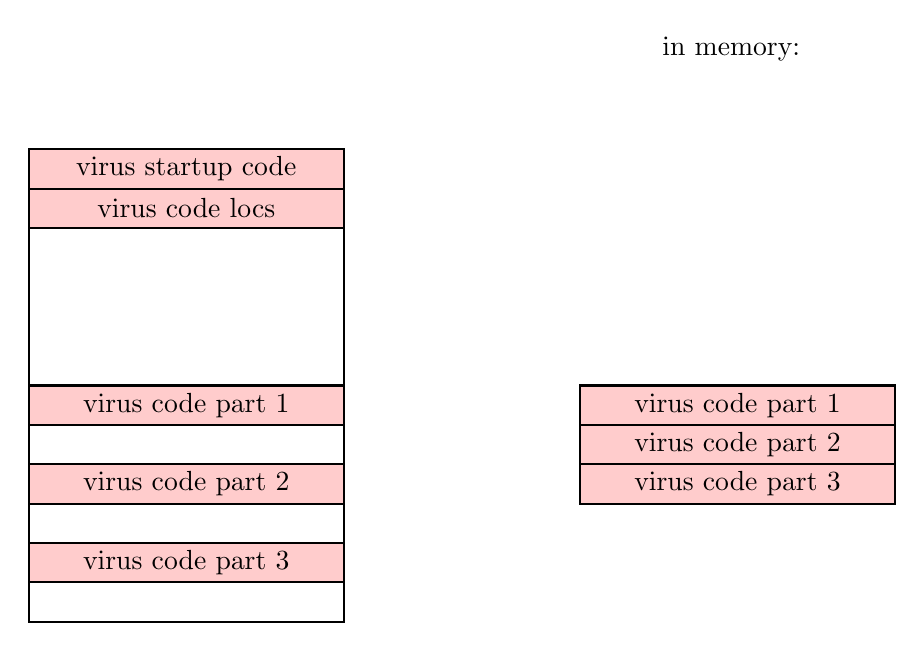
\begin{tikzpicture}
    \draw[fill=red!20,thick] (0, 0) rectangle (4, -0.5) node[midway] {virus startup code};
    \draw[fill=red!20,thick] (0, -0.5) rectangle (4, -1) node[midway] {virus code locs};
    \draw[thick] (0, -1) rectangle (4, -6);
    \draw[fill=red!20,thick] (0, -3) rectangle (4, -3.5)
        node[midway] {virus code part 1};
    \draw[fill=red!20,thick] (0, -4) rectangle (4, -4.5)
        node[midway] {virus code part 2};
    \draw[fill=red!20,thick] (0, -5) rectangle (4, -5.5)
        node[midway] {virus code part 3};
    \begin{scope}[xshift=7cm]
        \node[align=center,anchor=south] at (2, 1) { in memory: };
        \draw[fill=red!20,thick] (0, -3) rectangle (4, -3.5)
            node[midway] {virus code part 1};
        \draw[fill=red!20,thick] (0, -3.5) rectangle (4, -4)
            node[midway] {virus code part 2};
        \draw[fill=red!20,thick] (0, -4) rectangle (4, -4.5)
            node[midway] {virus code part 3};
    \end{scope}
    \end{tikzpicture}
\end{frame}

\begin{frame}{CIH cavities}
    \begin{itemize}
    \item gaps between sections
        \begin{itemize}
        \item common Windows linker aligned sections
        \item (align = start on address multiple of $N$, e.g. $4096$)
        \end{itemize}
    \item reassembling code avoids worrying about splitting instructions
    \end{itemize}
\end{frame}



\subsubsection{segment rounding}
\begin{frame}[fragile]{segment rounding}
\providecommand{\myemphA}[1]{\myemph<2>{#1}}
\providecommand{\myemphB}[1]{\myemph<3>{#1}}
objdump -x /bin/ls: 
\begin{Verbatim}[fontsize=\fontsize{9}{10},commandchars=\\\{\}]
   LOAD off    0x0000000000004000 vaddr 0x0000000000004000 paddr 0x0000000000004000 align 2**12
        filesz \myemphA{0x0000000000013091} memsz 0x0000000000013091 flags r-x
   LOAD off    \myemphB{0x0000000000018000} vaddr 0x0000000000018000 paddr 0x0000000000018000 align 2**12
        filesz 0x0000000000007458 memsz 0x0000000000007458 flags r--
\end{Verbatim}
running /bin/ls in gdb:
\begin{Verbatim}[fontsize=\fontsize{9}{10},commandchars=\\\{\}]
(gdb) info proc map
process 1178818
Mapped address spaces:
          Start Addr           End Addr       Size     Offset  Perms  objfile
      0x555555554000     0x555555558000     0x4000        0x0  r--p   /usr/bin/ls
      0x555555558000     0x55555556c000    \myemphA{0x14000}     0x4000  r-xp   /usr/bin/ls
      0x55555556c000     0x555555574000     0x8000    0x18000  r--p   /usr/bin/ls
....
\end{Verbatim}
\begin{itemize}
\item requested 0x13091 bytes, loaded 0x14000
\item x86-64 Linux: OS allocates only in one page = 4096-byte chunks
\end{itemize}
\end{frame}


\subsection{boot sector}

\againframe<5>{whereCode}

\usetikzlibrary{arrows.meta,chains}

\begin{frame}<1-2>[label=bootProc]{boot process}
    \begin{tikzpicture}
        \begin{scope}[start chain=going below,every node/.style={draw,align=center,join,on chain,thick,minimum width=3.5cm},
                      every join/.style={-Latex,thick}]
        \node[draw=none] (fixedLoc) { processor reset };
        \node[alt=<3>{draw=red,very thick}{}] (bios) {BIOS/EFI \\ \small (chip on motherboard)};
        \node[alt=<2>{draw=red,very thick}{}] (bootloader) {bootloader};
        \node[alt=<4>{draw=red,very thick}{}] (os) {operating system};
        \end{scope}
        \node[left=.5cm of bios,font=\small] (biosLabel) {very CPU/motherboard-specific code};
        \draw[-Latex,thick] (biosLabel) -- (bios);
        \node[left=.5cm of bootloader,font=\small,align=right] (bootloaderLabel) {fixed location on disk \\ code that understands files};
        \draw[-Latex,thick] (bootloaderLabel) -- (bootloader);
        \node[left=.5cm of os,font=\small] (osLabel) {files in a filesystem};
        \draw[-Latex,thick] (osLabel) -- (os);
    \end{tikzpicture}
\end{frame}

\begin{frame}{bootloaders in the DOS era}
    \begin{itemize}
    \item used to be common to boot from floppies
    \item \myemph{default to booting from floppy} if present
        \begin{itemize}
        \item even if hard drive to boot from
        \end{itemize}
    \item applications distributed as bootable floppies
    \item so bootloaders on all devices were a target for viruses
    \end{itemize}
\end{frame}

\begin{frame}{historic bootloader layout}
    \begin{itemize}
    \item bootloader in \myemph{first sector} (512 bytes) of device
    \item (along with partition information)
    \item code in BIOS to copy bootloader into RAM, start running
    \item bootloader responsible for disk I/O etc.
        \begin{itemize}
        \item some library-like functionality in BIOS for I/O
        \end{itemize}
    \end{itemize}
\end{frame}

\begin{frame}{bootloader viruses}
    \newcommand{\tearBox}{
        \draw[very thick] (0, -6) -- (0, 0) -- (4, 0) -- (4, -6);
        \draw[thick] (0, -6) -- (1.2, -5.5) -- (2., -6.6) -- (2.6, -5.8) -- (3.5, -6.6) -- (4, -6);
    }
    \begin{itemize}
    \item example: Stoned
    \end{itemize}
    \begin{tikzpicture}
        \draw[fill=green!20] (0, 0) rectangle (4, -.2);
        \draw[fill=yellow!20] (0, -.2) rectangle (4, -0.5) node[midway,font=\tiny] { partition table };
        \draw[fill=green!20] (0, -.5) rectangle (4, -1.0) node[midway,font=\small] { bootloader };
        \tearBox
        \begin{scope}[xshift=7cm]
        \draw[fill=red!20] (0, 0) rectangle (4, -.2);
        \draw[fill=yellow!20] (0, -.2) rectangle (4, -0.5) node[midway,font=\tiny] { partition table };
        \draw[fill=red!20] (0, -.5) rectangle (4, -1.0) node[midway,font=\small] { virus code };
        \begin{scope}[yshift=-4cm]
        \draw[fill=green!20] (0, 0) rectangle (4, -.2);
        \draw[fill=green!20] (0, -.5) rectangle (4, -1.0) node[midway,font=\small] { saved bootloader };
        \draw[dashed,fill=yellow!20] (0, -.2) rectangle (4, -0.5) node[midway,font=\tiny] { partition table (unused) };
        \end{scope}
        \tearBox 
        \end{scope}
        \draw[line width=1mm,black!50, -Latex] (4.2, -3) -- (6.8, -3);

        \begin{pgfonlayer}{bg}
            \begin{visibleenv}<2>
                \path[fill=blue!30] (0, -4) rectangle (4, -5) node[midway] { data here??? };
            \end{visibleenv}
        \end{pgfonlayer}
    \end{tikzpicture}
\end{frame}

\begin{frame}{data here???}
    \begin{itemize}
        \item might be data there --- risk
        \item some unused space after partition table/boot loader common
            \begin{itemize}
            \item (allegedly)
            \end{itemize}
        \item also be filesystem metadata not used on smaller floppies/disks
        \vspace{.5cm}
        \item but could be wrong --- oops
    \end{itemize}
\end{frame}

\begin{frame}{modern bootloaders --- UEFI}
    \begin{itemize}
    \item BIOS-based boot is going away (slowly)
    \item new thing: UEFI (Universal Extensible Firmware Interface)
    \item like BIOS:
        \begin{itemize}
        \item library functionality for bootloaders
        \item loads initial code from disk/DVD/etc.
        \end{itemize}
    \item unlike BIOS:
        \begin{itemize}
        \item much more understanding of file systems
        \item much more modern set of library calls
        \end{itemize}
    \end{itemize}
\end{frame}

\againframe<3>{bootProc}

\begin{frame}{BIOS/UEFI implants}
    \begin{itemize}
    \item infrequent
    \item BIOS/UEFI code is \myemph{very non-portable}
    \item BIOS/UEFI update may require physical access
    \item BIOS/UEFI code may require cryptographic signatures
    \item \ldots but \myemph{very hard to remove} --- ``persist'' other malware
    \item reports of BIOS/UEFI-infecting ``implants''
        \begin{itemize}
        \item sold by Hacking Team (Milan-based malware company) 
        \item listed in leaked NSA Tailored Access Group catalog
        \end{itemize}
    \end{itemize}
\end{frame}

\againframe<4>{bootProc}

\begin{frame}{system files}
    \begin{itemize}
    \item simpliest strategy: stuff that runs when you start your computer
    \item add a new startup program, run in the background
        \begin{itemize}
        \item easy to blend in
        \end{itemize}
    \vspace{.5cm}
    \item alternatively, infect one of many system programs automatically run
    \end{itemize}

    % FIXME: example from CodeRed or similar?
\end{frame}

 % FIXME: split out UEFI/Secure Boot section

\subsection{memory residence}


\begin{frame}{memory residence}
    \begin{itemize}
    \item malware wants to keep doing stuff
    \item one option --- background process (easy on modern OSs)
    \item also stealthy options:
        \begin{itemize}
        \item insert self into OS code
        \item insert self into other running programs
        \end{itemize}
    \end{itemize}
\end{frame}
 % FIXME: should have more extensive discussion of this somewhere

\section{virus: getting code invoked}


\begin{frame}<1-2>[label=invokeOptions]{invoking virus code: options}
    \begin{itemize}
    \item boot loader
    \item \myemph<2>{change starting location} 
    \item alternative approaches: ``entry point obscuring''
    \item \myemph<3>{edit code that's going to run anyways}
    \item \myemph<4>{replace a function pointer} (or similar)
    \item \ldots
    \end{itemize}
\end{frame}


\subsection{changing start location}


\begin{frame}[fragile,label=invokeStarting]{starting locations}
\begin{Verbatim}[fontsize=\fontsize{10}{11}\selectfont,commandchars=Q\{\}]
/bin/ls:     file format elf64-x86-64
/bin/ls
architecture: i386:x86-64, flags 0x00000112:
EXEC_P, HAS_SYMS, D_PAGED
start address Qmyemph{0x00000000004049a0}
\end{Verbatim}
    \begin{itemize}
    \item modern executable formats have `starting address' field
    \item just change it, insert jump to old address after virus code
    \end{itemize}
\end{frame}




\subsection{overwrite existing code}

\begin{frame}<1>[fragile,label=runAnyways]{run anyways?}
    \begin{itemize}
    \item add code at start of program (Vienna)
        \begin{itemize}
        \item \myemph<2>{plus restore replaced code after running malware code}
        \end{itemize}
    \item return with padding after it:
\begin{Verbatim}[fontsize=\fontsize{10}{11}\selectfont,commandchars=Q\{\}]
  404a01:       c3                      Qtextbf{retq}
  404a02:       0f 1f 40 00             nopl   0x0(%rax)
                Qtextit{replace with}
  404a01:       e9 XX XX XX XX          Qtextbf{jmpq    YYYYYYY}
\end{Verbatim}
        \begin{itemize}
        \item plus return after running malware code
        \end{itemize}
    \item any random place in program?
        \begin{itemize}
        \item just not in the \myemph{middle of instruction}
        \item and \myemph<2>{replace orignal code after running malware code}
        \end{itemize}
    \end{itemize}
\end{frame}

\begin{frame}[fragile,label=findValidChallenge]{challenge: valid locations}
    \begin{itemize}
    \item x86: probably don't want a full instruction parser
    \item x86: might be non-instruction stuff mixed in with code:
\begin{lstlisting}[language=myasm,style=smaller]
do_some_floating_point_stuff:
            movss float_one(%rip), %xmm0
            ...
            retq
float_one: .float 1
\end{lstlisting}
    \begin{itemize}
        \item floating point value one ({\tt 00 00 80 3f}) is not valid machine code
        \item disassembler might lose track of instruction boundaries
    \end{itemize}
    \end{itemize}
\end{frame}

\begin{frame}[fragile,label=findValidFindFunc]{finding function calls}
    \begin{itemize}
    \item one idea: replace calls
    \item normal x86 call FOO: {\tt E8 \textit{(32-bit value: PC - address of foo)}}
    \item could look for E8 in code --- \myemph{lots of false positives}
        \begin{itemize}
        \item probably even if one excludes out-of-range addresses
        \end{itemize}
    \end{itemize}
\end{frame}

\begin{frame}[fragile,label=findValidFindFunc2]{really finding function calls (1)}
\lstset{language=myasm,style=small}
    \begin{itemize}
    \item e.g. some popular compilers started x86-32 functions with
\begin{lstlisting}
foo:
    push %ebp       // push old frame pointer
    // 0x55
    mov %esp, %ebp  // set frame pointer to stack pointer
    // 0x89 0xec
\end{lstlisting}
    \item use to identify when {\tt e8} refers to real function
    \begin{itemize}
    \item (full version: also have some other function start patterns)
    \end{itemize}
    \end{itemize}
\end{frame}

\begin{frame}{really finding function calls (2)}
    \begin{itemize}
    \item x86-64 assembly seen a lot of ENDBR64 (hex {\tt f3 0f 1e fa})
    \item marker for valid locations to jump to
        \begin{itemize}
        \item intention: part of possible defense against return-oriented-programming-style attacks
        \item (we'll talk about what this means later)
        \end{itemize}
    \item likely only seen at beginning of functions, switch statement cases, etc.
    \end{itemize}
\end{frame}

\againframe<2>{runAnyways}

\begin{frame}{restoring replaced code?}
    \begin{itemize}
    \item Vienna: just write to memory addres
    \vspace{.5cm}
    \item modern OS: segfault/general protection fault
        \begin{itemize}
        \item code loaded read-only
        \end{itemize}
    \item easy solution: make library call to make it writable
        \begin{itemize}
        \item Linux: \texttt{mprotect}
        \item functionality exists to, e.g., allow compiling code at runtime
        \end{itemize}
    \end{itemize}
\end{frame}


\subsection{using dynamic linking features}

\begin{frame}{infecting shared libraries via relocations}
\begin{tikzpicture}
    \draw[thick] (0, 0) rectangle (4, -6) coordinate (bottomRight) node[midway] { \tt kernel32.dll };
    \draw[thick,fill=yellow!20] (0, 0) rectangle (4, -0.5) node[midway,font=\small] {header};
    \draw[thick,fill=blue!20] (0, -0.5) rectangle (4, -2.0);
    \node[font=\small,anchor=north] at (2, -0.5) {symbol table};
    \node[anchor=north west,font=\fontsize{9}{10}\selectfont] (GFAName) at (0, -0.9) {
        \tt GetFileAttributesA
    };
    \node[anchor=north west] at (GFAName.south west) {\tt \ldots};
    \draw[-Latex,thick] ([xshift=.5mm]GFAName.east) coordinate (startArrowA) -- ([xshift=.5cm]GFAName.west -| bottomRight) |- (3, -5);
    \fill[black] (startArrowA) circle[radius=.5mm];

    \draw[line width=2mm,-Latex,black!60] (4.6, -3) -- (6.9, -3);
    \begin{scope}[xshift=7cm]
    \draw[thick] (0, 0) rectangle (4, -6) coordinate (bottomRight) node[midway] { \tt kernel32.dll };
    \draw[thick,fill=yellow!20] (0, 0) rectangle (4, -0.5) node[midway,font=\small] {header};
    \draw[thick,fill=blue!20] (0, -0.5) rectangle (4, -2.0);
    \node[font=\small,anchor=north] at (2, -0.5) {symbol table};
    \draw[thick,fill=red!20] (0, -6) rectangle (4, -7) node[midway,font=\small] {virus code};
    \node[anchor=north west,font=\fontsize{9}{10}\selectfont] (GFANameB) at (0, -0.9) {
        \tt GetFileAttributesA
    };
    \node[anchor=north west] at (GFANameB.south west) {\tt \ldots};
    \draw[-Latex,very thick,red] ([xshift=.5mm]GFANameB.east) coordinate (startArrowA) -- ([xshift=.5cm]GFANameB.west -| bottomRight) |- (1, -6.2);
    \fill[red] (startArrowA) circle[radius=.5mm];
    \end{scope}
\end{tikzpicture}
\end{frame}

\begin{frame}{other dynamic-linking-based infections}
    \begin{itemize}
    \item could also modify
    \vspace{.5cm}
    \item relocations on executable
        \begin{itemize}
        \item this isn't the table entry for \texttt{puts}, \\ it's the one for \texttt{evilvirus}
        \end{itemize}
    \item list of needed libraries?
        \begin{itemize}
        \item the C standard library and virus.so
        \end{itemize}
    \item stubs and calls to stub
        \begin{itemize}
        \item very regular and easy to locate
        \end{itemize}
    \end{itemize}
\end{frame}
 % FIXME: 20.04 example?

% FIXME: discussion about hiding worm-like programs?

\section{virus summary?}


\begin{frame}{summary}
    \begin{itemize}
    \item how to hide:
        \begin{itemize}
        \item separate executable
        \item append
        \item existing ``unused'' space
        \item append + compression
        \end{itemize}
    \item how to run:
        \begin{itemize}
        \item change entry point (start address)
        \item change calls
        \item change beginning of function
        \item change dynamic-linking-related pointers
        \item arrange to run as part of OS
        \end{itemize}
    \end{itemize}
\end{frame}


\section{backup slides}
\begin{frame}{backup slides}
\end{frame}

\subsection{exercise}
\usetikzlibrary{chains}
\begin{frame}{exercise 1} 
\begin{tikzpicture}
\begin{scope}[start chain=going right,node distance=0mm,every node/.style={on chain,draw,font=\small,minimum height=1cm}]
\node (opcode) { opcode }; \node[dashed] { mod | reg{\fontsize{9}{10}\selectfont/opcode} | r/m}; \node[dashed] {scale / idx / base}; \node[dashed] {displacement}; \node[dashed] {immediate};
\end{scope}
\node[anchor=north west] (modrmtbl) at (opcode.south west) {
    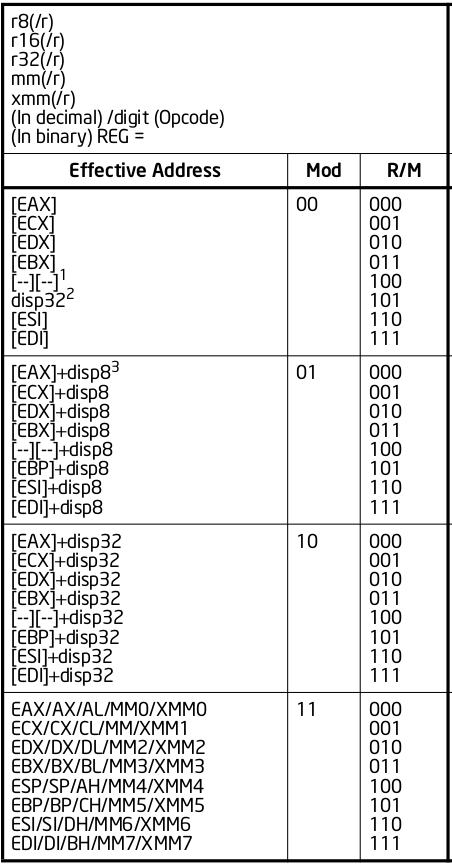
\includegraphics[height=0.8\paperheight]{../x8664-encoding/32bitmodrm}
};
\node[anchor=north west] (bts manual)at (modrmtbl.north east) {
    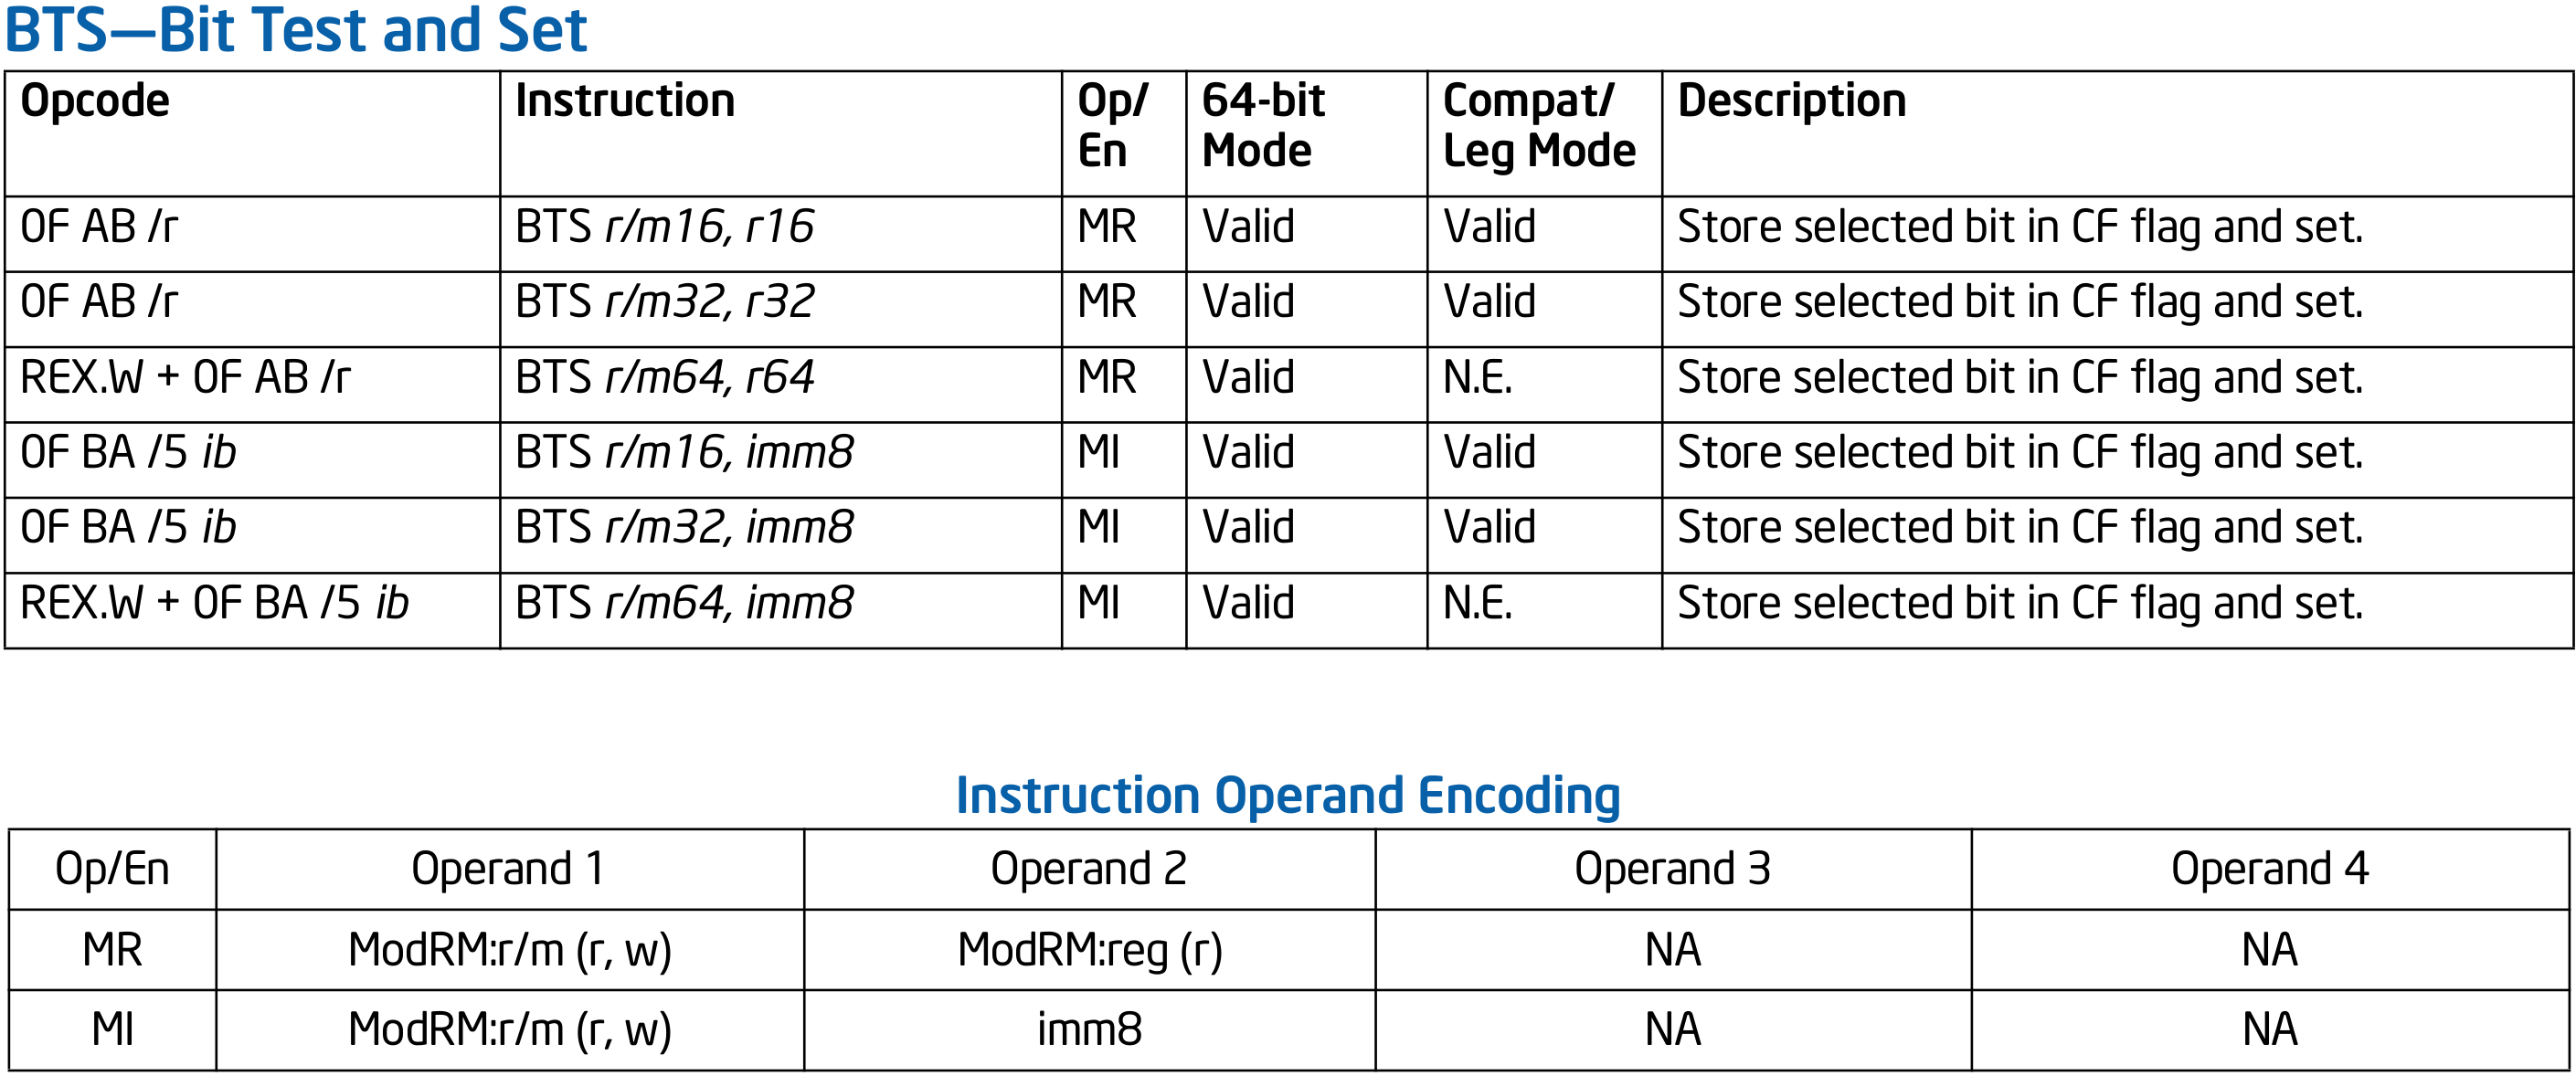
\includegraphics[width=0.75\textwidth]{../x8664-encoding/bts-manual}
};
\node[anchor=north west,align=left] (bts ex) at (bts manual.south west) {
    exercise: encode \texttt{btsl \$7, 4(\%rax)} \\
    (Intel syntax: \texttt{BTS DWORD PTR[RAX+4], 7})
};
\end{tikzpicture}
\end{frame}



\subsection{needed info encoding}

\providecommand{\myemphA}[1]{\myemph<1>{#1}}
\providecommand{\myemphB}[1]{\myemph<2>{#1}}
\providecommand{\myemphAB}[1]{\myemph<1-2>{#1}}
\providecommand{\myemphC}[1]{\myemph<3>{#1}}
\begin{frame}[fragile,label=dynLinkNeeded2]{dynamic linking: what to load? (2)}
\begin{itemize}
\item excerpt from {\tt objdump -sx hello.exe}:
\end{itemize}
\begin{Verbatim}[commandchars=@\{\},fontsize=\fontsize{9}{10}\selectfont]
Program Header:
@textit{...}
 DYNAMIC off    0x0000000000002e20 vaddr @myemph{0x0000000000403e20} paddr 0x0000000000403e20 align 2**3
         filesz 0x00000000000001d0 memsz 0x00000000000001d0 flags rw-
@textit{...}
Dynamic Section:
  @myemphAB{NEEDED               libc.so.6}
  @myemphC{INIT                 0x0000000000401000}
  ...
  @myemphB{STRTAB}               0x0000000000400420
  ...
@textit{...}
 @myemphAB{403e20} @myemphA{01000000 00000000} @myemphB{01000000 00000000}  ................
 403e30 @myemphC{0c000000 00000000 00104000 00000000}  ..........@.....
\end{Verbatim}
\hrule
type \myemphA{0x1 = ``DT\_NEEDED''} (from ELF manual)\\
value \myemphB{0x1 = string table entry 1} \\
\hrule
type \myemphC{0xC = ``DT\_INIT''} \\
value \myemphC{0x401000} \\
\end{frame}



\subsection{static symbol/relocation tables}
\begin{frame}[fragile,label=linkingExAsm]{hello.s}
\begin{lstlisting}
.data
string: .asciz "Hello, World!"
.text
.globl main
main:
    movq $string, %rdi
    call puts
    ret
\end{lstlisting}
\end{frame}

\begin{frame}[fragile,label=linkingExObjRepeat]{hello.o (pre-static or dynamic linking)}
\begin{Verbatim}[commandchars=\\\{\},fontsize=\fontsize{9}{10}\selectfont]
SYMBOL TABLE:
0000000000000000 l    d  .text  0000000000000000 .text
0000000000000000 l    d  .data  0000000000000000 .data
0000000000000000 l    d  .bss   0000000000000000 .bss
0000000000000000 l       .data  0000000000000000 string
0000000000000000 \myemphSix{g}       \myemphSeven{.text  0000000000000000} main
0000000000000000         \myemphTwo{*UND*  0000000000000000 puts}

RELOCATION RECORDS FOR [.text]:
OFFSET           TYPE              VALUE 
0000000000000003 \myemphFive{R_X86_64_32S}      \myemphFour{.data}
0000000000000008 \myemphFive{R_X86_64_PC32}     \myemphThree{puts}-0x0000000000000004
\end{Verbatim}
\begin{tikzpicture}[overlay,remember picture]
    \tikzset{overBox/.style={at=(boxLoc),anchor=center,align=center,draw,rectangle,fill=white}}
    \coordinate (boxLoc) at ([yshift=-2.5cm]current page.center);
    \begin{visibleenv}<2>
        \node[overBox] {
            undefined symbol: look for {\tt puts} elsewhere
        };
    \end{visibleenv}
    \begin{visibleenv}<3>
        \node[overBox] {
           insert address of puts, format for {\tt call}
        };
    \end{visibleenv}
    \begin{visibleenv}<4>
        \node[overBox] {
           insert address of string, format for {\tt movq}
        };
    \end{visibleenv}
    \begin{visibleenv}<5>
        \node[overBox] {
            different ways to represent address \\
            {\tt 32S} --- signed 32-bit value \\
            {\tt PC32} --- 32-bit difference from current address
        };
    \end{visibleenv}
    \begin{visibleenv}<6>
        \node[overBox] {
            {\tt g}: global --- used by other files \\
            {\tt l}: local 
        };
    \end{visibleenv}
    \begin{visibleenv}<7>
        \node[overBox] {
            {\tt .text} segment beginning plus 0 bytes
        };
    \end{visibleenv}
\end{tikzpicture}
\end{frame}

\begin{frame}[fragile]{hello.o / statically linked, no PIE}
hello.o:
\begin{Verbatim}[commandchars=\\\{\},fontsize=\fontsize{9}{10}\selectfont]
Disassembly of section .text:

0000000000000000 <main>:
   0:   48 c7 c7 00 00 00 00    mov    $0x0,%rdi
                        3: R_X86_64_32S .data
   7:   e8 00 00 00 00          call   c <main+0xc>
                        8: R_X86_64_PLT32       puts-0x4
   c:   c3                      ret    
\end{Verbatim}
\hrule
hello.exe (gcc -static -no-pie):
\begin{Verbatim}[commandchars=\\\{\},fontsize=\fontsize{9}{10}\selectfont]
Disassembly of section .text:
...
 00000000004016c3 <main>:
   4016c3:▶      48 c7 c7 b5 16 40 00 ▶  mov    $0x4016b5,%rdi
   4016ca:▶      e8 e1 a9 00 00       ▶  call   40c0b0 <_IO_puts>
   4016cf:▶      c3                   ▶  ret    
...
\end{Verbatim}
\end{frame}




\section{floationg point calling convention}

\begin{frame}{floating point calling convention}
    \begin{itemize}
    \item use {\tt \%xmm} registers in order
    \end{itemize}
\end{frame}

\begin{frame}[fragile,label=variadic]{note: variadic functions}
    \begin{itemize}
    \item variable number of arguments
        \begin{itemize}
        \item {\tt printf}, {\tt scanf}, \ldots
        \item see {\tt man stdarg}
        \end{itemize}
    \vspace{.5cm}
    \item same as usual 
    \item \ldots but \lstinline|%rax| contains number of {\tt \%xmm} used
    \end{itemize}
\end{frame}


\section{exploring assembly/optimization effects}

\begin{frame}{exploring assembly}
\begin{itemize}
\item compiling little C programs looking at the assembly is nice:
\item {\tt gcc -S \myemph<2>{\textbf<2>{-O}}}
    \begin{itemize}
    \item extra stuff like {\tt .cfi} directives (for try/catch)
    \end{itemize}
\vspace{.5cm}
\item or disassemble:
\item {\tt gcc \myemph<2>{\textbf<2>{-O}} -c file.c} (or make an executable)
\item {\tt objdump -dr file.o} (or on an executable) 
    \begin{itemize}
    \item d: disassemble
    \item r: show (non-dynamic) relocations
    \end{itemize}
\end{itemize}
\end{frame}

\begin{frame}[fragile,label=noOpt]{assembly without optimizations}
\begin{itemize}
\item compilers do \myemph{really silly things} without optimizations:
\begin{lstlisting}[language=C, style=smaller]
int sum(int x, int y) { return x + y; }
\end{lstlisting}
\vspace{-.125cm}
\begin{lstlisting}[language=myasm,style=smaller]
sum:
    pushq   %rbp
    movq    %rsp, %rbp
    movl    %edi, -4(%rbp)
    movl    %esi, -8(%rbp)
    movl    -4(%rbp), %edx
    movl    -8(%rbp), %eax
    addl    %edx, %eax
    popq    %rbp
    ret
\end{lstlisting}
\vspace{-.3cm}
\item instead of {\tt gcc -O} version:
\vspace{-.1cm}
\begin{lstlisting}[language=myasm,style=smaller]
sum:
    leal (%rdi,%rsi), %eax
    ret
\end{lstlisting}
\end{itemize}
\end{frame}



    % FIXME: exercise
\section{caller/callee saved}

\begin{frame}{caller-saved registers}
    \begin{itemize}
        \item functions \myemph{may} freely \myemph{trash} these
        \vspace{.5cm}
        \item return value register {\tt \%rax}
        \item argument registers: \\
            \begin{itemize}
            \item {\tt \%rdi}, {\tt \%rsi}, {\tt \%rdx}, 
              {\tt \%rcx}, {\tt \%r8}, {\tt \%r9}
              \end{itemize}
        \item \%r11
        \item MMX/SSE/AVX registers: {\tt \%xmm0-15}, etc.
        \item floating point stack: {\tt \%st(0)-\%st(7)}
        \item condition codes (used by {\tt jne}, etc.)
    \end{itemize}
\end{frame}

\begin{frame}[fragile,label=calleeSaved]{callee-saved registers}
    \begin{itemize}
    \item functions \myemph{must preserve} these
    \vspace{.5cm}
    \item {\tt \%rsp} (stack pointer), {\tt \%rbp} (frame pointer, maybe)
    \item {\tt \%r12-\%r15}
    \end{itemize}
\end{frame}

\begin{frame}[fragile,label=callerCallee]{caller/callee-saved}
\lstset{style=small}
\begin{lstlisting}
foo:
    pushq %r12 // r12 is caller-saved
    ... use r12 ...
    popq %r12
    ret

...
other_function:
    pushq %r11 // r11 is caller-saved
    ...
    callq foo
    popq %r11
\end{lstlisting}
\end{frame}

% XXX enter/leave ???




\end{document}
